\documentclass{article}
\usepackage[UTF8]{ctex}
\usepackage{listings}

\usepackage{graphicx,amsmath,amssymb,amsthm, boxedminipage,xcolor,subfigure}

\usepackage{algorithm}
\usepackage{algpseudocode}


\newtheorem{theorem}{Theorem}[section]
\newtheorem{proposition}[theorem]{Proposition}
\newtheorem{lemma}[theorem]{Lemma}
\newtheorem{corollary}[theorem]{Corollary}
\newtheorem{definition}[theorem]{Definition}

\newtheorem*{theorem*}{Theorem}
\newtheorem*{lemma*}{Lemma}
\newtheorem*{proposition*}{Proposition}

\newcommand{\E}{\mathbb{E}}
\newcommand{\scalar}[2]{\ensuremath{\langle #1, #2\rangle}}
\newcommand{\floor}[1]{\left\lfloor #1 \right\rfloor}
\newcommand{\ceil}[1]{\left\lceil #1 \right\rceil}
\newcommand{\norm}[1]{\|#1\|}
\newcommand{\pfrac}[2]{\left(\frac{#1}{#2}\right)}
\newcommand{\nth}[1]{#1^{\textsuperscript{th}}}
\newcommand{\core}{\textnormal{core}}





\newcommand{\poly}{\textnormal{poly}}
\newcommand{\quasipol}{\textnormal{quasipol}}
\newcommand{\ssubexp}{\textnormal{stronglySubExp}}
\newcommand{\wsubexp}{\textnormal{weaklySubExp}}
\newcommand{\simplyexp}{\textnormal{E}}
\newcommand{\expo}{\textnormal{Exp}}



\newcommand{\N}{\mathbb{N}}
\newcommand{\nn}{\mathbb{N}_0^n}
\newcommand{\R}{\mathbb{R}}
\newcommand{\Z}{\mathbb{Z}}

\definecolor{darkgreen}{rgb}{0,0.6,0}


\title{Algorithm}
\author{Little0o0,lzl,jyh,cjz}
\date{\today}

\begin{document} 


\maketitle

\section{Introduction}
    NULL

\section{数学归纳法} 
\subsection{PPT}
    \subsubsection{}对任意的自然数$x(x \ne 1$)和$n$,$x^{n}
-1$能被$x-1$除尽
    \paragraph{Hint:} c$(x^{n-1}-1)x = x^{n} - x = x^{n} - 1 + (x - 1) $

    \subsubsection{}前n个自然数之和为$\frac{n(n+1)}{2}$
    \paragraph{Hint:} 若$\sum_{i=1}^{n-1} = \frac{n(n-1)}{2}$, $\sum_{i=1}^{n} =\sum_{i=1}^{n-1} + n = \frac{n(n-1)}{2} + n = \frac{n(n+1)}{2}$
    
    \subsubsection{}级数$8+13+18+23+…+(3+5n)$之和是$2.5n^{2}+5.5n$
    \paragraph{Hint:} 若$8+13+18+23+…+(3+5(n-1)) = 2.5(n-1)^{2}+5.5(n-1)$,$8+13+18+23+…+(3+5n) = 2.5(n-1)^{2}+5.5(n-1) + 3+5n = 2.5n^{2}+ 0.5n -3 + 5n +3 = 2.5n^{2}+5.5n $
    
    \subsubsection{}若n是自然数,且$1+x>0$,则$(1+x)^{n}\geq 1+nx $。
     \paragraph{Hint:}若$(1+x)^{n-1}\geq 1+nx-x$,$(1+x)^{n} \geq (1+nx-x)(1+x) = 1+nx+(n-1)x^{2}  \geq 1+nx$
     
     \subsubsection{}平面上n条居一般位置的直线能把平面分割成多少块区域?
     \paragraph{Hint:}只需证明第n+1条直线分割了n+1个区域。先把第n条直线移去,由于没有第n条直线,第n+1条直线会增加n个区域,再把n放回去,那么n和n+1一定会在某个区域的某一点相交,而且这两条直线都分割了这个区域,所以这个区域被分成了4个部分,在有第n条直线的时候,第n+1条直线把这个区域多分了两个部分而不是一个,得证。
     
     \subsubsection{}证明平面上任意条直线构成的区域可以仅使用两种颜色有效着色,使得相邻的两个区域不同色。
     \paragraph{Hint:}若n-1可以, 在添加第n条直线的时候,根据保留直线的一侧的着色,翻转另一侧。
     
     \subsubsection{}考察下面的三角形。\\
\indent \indent \indent \indent 1 = 1 \\
\indent \indent \indent3 + 5 = 8\\
\indent \indent 7+ 9 +11 = 27\\
\indent13+15+17+19 = 64\\
21+23+25+27+29 = 125\\
证明:上述三角形中第i行的和是$i^{3}$
     \paragraph{Hint:}  转为证明第i行最后一个数是$i^{2}+i-1$,然后直接求和。
     
     \subsubsection{}证明$\sum^{n}_{i=1}(\frac{1}{2})^{i}< 1$ 
     \paragraph{Hint:}转为证明$\sum^{n-1}_{i=1}(2)^{i}< 2^{n}$
     
    老师希望的应该是通过$\sum^{n+1}_{i=1}(\frac{1}{2})^{i} = \frac{1}{2}+\frac{1}{2}\sum^{n}_{i=1}(\frac{1}{2})^{i} < \frac{1}{2} + \frac{1}{2} * 1 = 1$来证明
     
     \subsubsection{}证明任意一张连通平面图的节点数(V)、边数(E)和面数(F)的关系可由公式V+F=E+2表示。
     \paragraph{Hint:双重归纳法}首先对节点数归纳,再对面数归纳。\\
     1. 若只有一个面,即在树中, V = E + 1.(若n个节点的树有n-1条边,而n+1个节点的树至少有一个节点的度为1,删掉后成为n个节点的树)\\
     2.对面数归纳,即 证V + n = E + 2. 若 n 满足, 在n + 1 时,一定存在某个面和最外面那个面相邻,删除相邻的那条边,图仍然连通,这样就减少了一个面和一条边, 定理得证。
     
     \subsubsection{}令G=(V,E)是一个有向图。证明G中存在一个独立集(任意两点都不相邻的点构成的集合)S(G)使得G中的每一个结点都可以从S(G)的某一个结点通过一条长度不超过2的路可达。
     \paragraph{Hint:}假定对任意任何节点数小于n的图都成立,对节点数为n的图G,对任意节点v,令$N(v) = \{v\} \cup \{w\in V| (v,w)\in E\}$(v 指向 w ), H 为删去N(v)后的图,S(H)为其的独立集。\\
     1.若$S(H) \cup \{v\}$ 是独立的,那么$S(G) = S(H) \cup \{v\}$\\
     2.若$S(H) \cup \{v\}$ 不是独立的,那么说明S(H) 中肯定有指向v的点,$S(G) = S(H)$
     
     \subsubsection{}令G=(V,E)是连通的无向图,O是V中度数为奇数的结点的集合,证明可以把O中的结点分成结点对,在每一对中都能找到连接这两个结点的无重边的路。(如果两条路不包含相同的边,则是无重边的路)
     \paragraph{Hint:}(加强归纳假设),假设对边数小于n的无向图成立,在边数为n的时候,把各个连通分支单独考虑,都能生成节点对,在任意一个连通分支上的任意两个节点,去掉一条连接这两个节点的路,进行归纳假设。在剩余的图中一定能生成节点对,任意一个节点对都能找到无重边的路,最后把去掉的那条路加上即可。注意的是路上的节点度数奇偶性不回改变,若两端节点变成奇,则添加这两个节点对,若变成偶数,则合并之前的两个节点对,并且把这条路加上。\\
     \textbf{注意:}这题没有假设对边数小于n的\textbf{连通}无向图成立,因为删除以后可能不连通,属于增强归纳假设。
    
     \subsubsection{}证明数学平均数大于几何平均数
     \paragraph{Hint:逆向归纳法}如果命题P对某个自然数的无穷子集成立,且P对n成立能推出其对n-1成立,那么P对任意自然数都成立。\\
     即先证明对$n = 2^{k}$成立(易证),再通过对n成立的话能够推出对n-1成立,就能得证。\\
     第二步证明方法如下:\\
     令$z =\frac{\sum^{n-1}_{i=1}x_{i}}{n-1}$, 则若已知n时成立,有$x_{1}x_{2}\dots x_{n-1}z \leq\frac{\sum^{n}_{i=1}x_{i} + z}{n} = \frac{(n-1)z+z}{n} = z$. 所以,$x_{1}x_{2}\dots x_{n-1} \leq z^{n-1}$. $(x_{1}x_{2}\dots x_{n-1})^{\frac{1}{n-1}
     }\leq z$ 。得证

     
     \subsection{Homework}
     
     \subsubsection{}数列1,2,3,4,5,10,20,40,…,该数列开始是等差数列,第5项以后为等比数列,证明任意一个正整数都可表示为这个数列中的不同数之和。
     \paragraph{Hint:}从5开始,所有5的倍数都可以用数列中5后面的数表示(二进制),两个相邻的5的倍数之间用1,2,3,4填充
     
     \subsubsection{}广场上站着99个间谍,间谍与间谍之间的距离互不相等,每个间谍都盯着离自己最近的那个间谍看,证明总存在一个没被人盯着的间谍。
     \paragraph{Hint:}数学归纳法证明对任意2m-1个间谍都满足\\
     3个显然满足,对于2m+1,找出这些人中距离最近的两个人,它们必定相互盯着,由归纳假设,剩下2m-1个人中必定有一个没有被盯着。
     
     
     \subsubsection{}有10个海盗抢得了100枚金币,每个海盗都能够很理智地判断自己的得失,他们决定这样分配金币: \\
1)按照强壮与否排序,其中最强壮的人为1号,以此类推,最瘦小的人为10号。\\
2)先由1号提出分配方案,然后由所有人表决,当且仅当等于或多于半数人(包括自己)同意时,方案才算被通过,否则他将被扔入大海喂鲨鱼;\\
3)如果1号死了,将由2号提方案,其余的人表决,当且仅当超过半数(包括自己)同意时,方案才算通过,否则2号同样将被扔入大海喂鲨鱼;\\
4)往下以此类推…… \\
海盗们都很精明,他们首先会尽量保住自己的命,其次在保住命的前提下都想分到尽可能多的金币,而且他们也很希望自己的同伴喂鲨鱼。假如你是那个1号海盗,你将怎样分配,才能既保住命,又能分到最多的金币?最多能分到多少呢?\\
如果还是100枚金币,但海盗的数量是20,50,100,200,400又该怎么样呢?
     \paragraph{Hint:}在200以内,第n个海盗对其他人的分配方案是上一个的取反再把上一个置0。202以后都是0个
     
     
     \section{算法分析}
     \subsection{PPT}
     NULL
     
      \subsection{Homework}
     
     \subsubsection{} 证明$log(n) = O(n^{k})$,k为正常数
     \paragraph{Hint:}根据定理3.1$(f(n))^{c}=O(a^{f(n)})$ 令$c = 1, f(n) = klog(n)$.
     
     \subsubsection{}寻找单调递增函数f(n)和g(n),使得f(n)=O(g(n))和g(n)=O(f(n))都不成立
     \paragraph{Hint:}构造两个函数,对于偶数,一个增长较快,对于奇数,另一个增长较快

$$ f(x)=\left\{
\begin{aligned}
f(n-1) +1 &  &odd\\
f(n-1)+g(n-1)^{2}&  & even\\
\end{aligned}
\right.
$$

$$g(x)=\left\{
\begin{aligned}
g(n-1) +1 &  & even\\
g(n-1)+f(n-1)^{2}&  &odd\\
\end{aligned}
\right.
$$
     
     \subsubsection{}假设解决同一个问题的两个算法A1和A2的时间复杂性分别为$O(n^{3})$和O(n),如果为这两个算法分别编写程序并在同样的环境下运行,算法A2的程序一定比算法A1的程序运行得快吗?为什么?
     \paragraph{Hint:}不一定
     
     \subsubsection{}考虑以下冒泡排序算法,1)元素比较的最少次数是多少?何时达到最小值?2)元素比较的最多次数是多少?何时达到最大值?3)可以用$O,\Theta,\Omega$表示算法的运行时间吗?
     
    \lstset{language=C}
    \begin{lstlisting}
    算法BubbleSort
    输入:n个元素的数组A[1..n]
    输出:按非降序排列的数组A[1..n]
    1. i=1, sorted=false
    2. while i<=n-1 and not sorted
    3.    sorted=true
    4.    for j=n downto i+1
    5.        if A[j]<A[j-1] 
    6.            交换A[j]与A[j-1]
    7.            sorted=false
    8.        end if
    9.    end for
    10.   i=i+1
    11.end while
    \end{lstlisting}
     
     \paragraph{Hint:}最少次数为n-1,有序的时候,最多为$\frac{n(n-1)}{2}$,反序的时候。(第三问不是很会答)
     
     \subsubsection{}证明$\sum^{n}_{i=1} = \theta(logn)$
     \paragraph{Hint:}根据求和的积分近似$\int^{n}_{m-1}f(x)dx \leq \sum^{n}_{j=m}f(j) \leq \int^{n+1}_{m}f(x)dx$
     
     \subsubsection{}设有如下递推关系:
     $$ T(n)=\left\{
    \begin{aligned}
    T(\frac{n}{2}) +1 &  &even\\
    2T(\frac{n-1}{2})&  & odd\\
    \end{aligned}
    \right.
    $$
    其中T(1)=1。\\
1)证明当$n=2^k$时,T(n)=O(logn)\\
2)证明存在无穷集合X,当$n \in X$时,$T(n)=\Theta(n)$\\
3)以上两个结论说明了什么?\\
        
     \paragraph{Hint:}1)对于$n=2^k$时,则$T(n) = T(\frac{n}{2}) +1$,故$T(n) = k = log n $。\\
     2)考虑$n = 2^{k}-1$,$T(2^{k}-1) = 2^{k} -1$\\
     3)不知道
     
     \subsubsection{}求解递推关系式$T(n) = n + \sum ^{n-1}_{i=1}T(i)$,其中T(1)=1
     \paragraph{Hint:}暴力计算$T(n) = n + n-1 + 2*(n-2)+4*(n-3)+\dots + 2^{n-1}*1$然后错位相减。
     
     \section{基于归纳的算法设计}
     \subsection{PPT}
     
     \subsubsection{}给定一串实数$an,a_{n-1},…,a_1,a_0$,和一个实数x,计算多项式$P_{n}(x)=a_{n}x^{n}+a_{n-1}x^{n-1}+…+a_{1}x+a_{0}$的值
     \paragraph{Hint:}(1).直接$P_{n}(x)= P_{n-1}(x)+a_{n}x^{n}$需要n(n+1)/2次乘法和n次加法运算。\\
    (2)更强的归纳假设:已知如何计算多项式$P_{n-1}(x)$的值,也知道如何计算$x_{n-1}$。\\
    计算$x_{n}$仅需要一次乘法,然后再用一次乘法得到$a_{n}x_{n}$,最后用一次加法完成计算,总共需要2n次乘法和n次加法。\\
    (3)归纳假设(翻转了顺序的):已知如何计算$P'_{n-1}(x) = =a_{n}x^{n-1}+a_{n-1}x^{n-2}+…+a_{1}$(这不是导数的意思!)\\
    $P'_{n}(x) = xP'_{n-1}(x)+a_{0}$,该算法仅需要n次乘法和n次加法,以及一个额外的存储空间。\\
    
     \subsubsection{}令G=(V,E)是一个无向图。一个G的导出子图是一个图H=(U,F),满足$U \subseteq V$且U中两顶点若在E中有边则该边也包含在F中。\\
     问题:给定一个无向图G=(V,E)和一个整数k,试找到G的一个最大规模的导出子图H=(U,F),其中H中所有顶点的度$\geq$k,或者说明不存在这样的子图。\\

     \paragraph{Hint:}任何度<k的顶点都可以被删除。删除的次序并不重要。这种删除是必须的,而删除后剩下的图必定是最大的(没给出正确性证明)\\
     
     \subsubsection{}问题:给定一个集合A和一个从A到自身的映射f,寻找一个元素个数最多的子集$S \subseteq A$,S满足:\\
     (1) f把S中的每一个元素映射到S中的另一元素(即,f把S映射到
它自身),\\
(2) S中没有两个元素映射到相同的元素(即,f在S上是一个一
对一函数)。
     \paragraph{Hint:}归纳假设:对于包含n-1个元素的集合,如何求解问题是已知的。\\
假定有一个包含n个元素的集合A,并且要寻找一个满足问题
条件的子集。任何没有被其它元素映射到的元素i,不可能属于S。则我们简单地把它从集合中删除。现在我们得到集合A/=A-{i},其元素个数为n-1,
由归纳假设,我们已知对A/如何求解。如果不存在这样的一个i,则映射是一对一的,即为所求,结束。\\
     \lstset{language=C}
    \begin{lstlisting}
    Algorithm Mapping(f,n)
Input: f (an array of integers whose values are between 1 to n)
Output: S (a subset of the integers from 1 to n, such that f is one-to-one on S)
begin
    S:=A; {A is the set of numbers from 1 to n}
    for j:=1 to n do c[j]:=0;
    for j:=1 to n do increment c[f[j]];
    for j:=1 to n do
        if c[j]=0 then put j in Queue;
    while Queue is not empty
        remove i from the top of the queue;
        S:=S-{i};
        decrement c[f[i]];
    if c[f[i]]=0 then put f[i] in Queue
end
    \end{lstlisting}
     总共的步骤数是O(n)
     
     \subsubsection{}在n个人中,一个被所有人知道但却不知道别人的人,被定义为社会名流。找到这个社会名流。
     \paragraph{Hint:}最坏情况下可能需要问n(n-1)个问题。\\
        问题:给定一个$n\times n$邻接矩阵,确定是否存在一个i,其满足在第i列所有项(除了第ii项)都为1,并且第i行所有项(除了第ii项)都为0。\\
        算法如下:问A是否知道B,并根据答案删除A或者B。假定删
除的是A。则由归纳法在剩下的n-1个人中找到一个社会名流。如果没有社会名流,算法就终止;否则,我们检测A是否知道此社会名流,而此社会名流是否不知道A\\
算法被分为两个阶段:\\
1)通过消除只留下一个候选者,\\
2)检查这个候选者是否就是社会名流。\\
至多要询问3(n-1)个问题:\\
第一阶段的n-1个问题用于消除n-1个人,而为了验证侯选者就是社会名流至多要2(n-1)个问题。\\
     
     \subsubsection{}给定一个精确的位置以及在城市中几座矩形建筑的外形,画出这些建筑的二维轮廓并且消去隐藏线。
     \paragraph{Hint:}分治法,合并时从左到右同时扫描两个轮廓。在最坏情况下完整的算法运行时间是O(nlogn)。
     
     
     \subsubsection{}令T是一个根为r的二叉树。节点v的高度是v和树下方最远叶子的距离。节点v的平衡因子被定义成它的左子树的高度与右子树的高度的差。\\
     问题:给定一个n个节点的二叉树T,计算它的所有节点的平衡
因子。\\
     \paragraph{Hint:}通过对节点数<n的二叉树的全部节点的平衡因子和\textbf{高度}。进行归纳假设。
     
     
     
     \subsubsection{}问题:给定实数序列$x_{1},x_{2},…,x_{n}$
(不需要是正数),寻找连续子序列$x_{i},x_{i+1},…,x_{j}$,使得其数值之和在所有的连续子序列数值之和中为最大。称这个子序列为最大子序列。,只能扫描一次。
     \paragraph{Hint:}去掉最后一个$x_{n}$,如果$x_{n}$为负数,就把它丢掉。然后继续在剩下n-1个元素(S')中招最大子序列,如果其最大子序列是最后一个j=n-1, 则把$x_{n}$包含进去,如果j<n-1,则存在两种情况,一种是S'中的元素最大子序列已经是最大,另一种是还存在一个子序列,在在S
'中不是最大,但是加入$x_{n}$是最大。\\
更强的归纳假设:已知如何找到规模<n的序列的最大子序列,以及作为后缀的最大子序列。(即是一个后缀)\\
\\
BUT:为什么不从左到右扫描求和,当和成为负数的时候就舍弃前面部分呢?\\
     \subsubsection{}给定一个整数K和n个不同大小的物品,第i个物品的大小为整数ki,寻找一个物品的子集,它们的大小之和正好为K,或者确定不存在这样的子集。
     \paragraph{Hint:}动态规划打表若已知$P(n-1,k),k\in K$,则可以求出$P(n,k),k\in K$,总复杂度O(nK).
      \subsection{homework}
      
     \subsubsection{}在寻找一对一映射问题中,算法结束时集合S是否可能为空集?请证明你的结论。
     \paragraph{Hint:}如果为空集,那最后一个节点所指向的节点不应该在它之前被删除。
     
     \subsubsection{}写出轮廓问题的伪代码
     \paragraph{Hint:}懒得写了,有空填坑
     
     \subsubsection{}有A、B、C三个桩子,A上放有n个不同大小的圆盘,按大小递减顺序自下而上。1)设计算法,用最少的移动步数将A上的圆盘都移到C,每次只能移一个,且任一桩子上的圆盘都必须满足圆盘大小自下而上递减的顺序。2)给定数组p,其元素取值只有1,2,3三种,代表了n个圆盘目前的位置,1代表A,2代表B,3代表C,p[i]的值为第i个圆盘的位置。例如p={3,3,2,1}表示共有4个圆盘,第一个和第二个都在C,第三个在B,第4个在A。如果p代表了1)中的最优移动过程中某一步的状态,则求出这是第几步。注意诸如p=[2,2]是不可能出现的,此时算法得到-1
     \paragraph{Hint:}1)汉诺塔递归求解。\\
     2)从最大的一个盘,即第n个盘开始考虑,若p[n] = 1, 则该盘还未移动过,考虑前n-1个盘,若p[n]=2返回-1\\
     对盘1到i来说,如果目标是从src到dst,则类似考虑:\\
     若p[i]=src,考虑1到i-1的盘的情况,这i-1个盘的目标是从src到mid\\
     若p[i]=dst,已移动$2^{i-1}$步,考虑1到i-1的盘,它们此时处于从mid到dst的过程中\\
     若p[i]=mid,返回-1\\
     
     \subsubsection{}课上的最大连续子序列是指和最大,如果要求是积最大呢?设空序列的积为1,只需求出最大值即可,不需要知道是哪个序列
     \paragraph{Hint:}问题的解与最大子序列相似,但需要增强归纳假设。可假定我们知道:(1)乘积最大子序列;(2)乘积最大后缀;(3)有着最小负乘积的子序列;(4)有着最小负乘积的后缀。算法和最大子序列相似。
     
     \subsubsection{}背包问题中如果各种大小的物品的数量不限,那么如何知道背包是否能够恰好放满?
     \paragraph{Hint:}修改原来的算法,仍然是动态规划打表法。
     
     \subsubsection{}设计算法将1到$n^{2}$按顺时针方向由内而外填入一个n*n的矩阵。
     \paragraph{Hint:}简单递归,选取左上角的点为基准点,按照层数从外到内进行递归。或者从内到外进行递归。
     
     \subsubsection{}给定整数数组A[1..n],相邻两个元素的值最多相差1。设A[1]=x,A[n]=y,并且x<y,输入z,x,y,判断z在数组A中出现的位置。给出算法及时间复杂性(不得穷举)
     \paragraph{Hint:}从左到右扫描,跳到之后当前数字减去z的绝对值的位置处,当绝对值为0就记录位置。\\
     如果题目要求的是找到一个z的位置,就只要用二分法查找则可。\\
     
     \subsubsection{}用分治法找到数组中的最大数和最小数,若数组规模为2的幂,证明需要的比较次数为3n/2-2。
     \paragraph{Hint:}等着填坑
     
     \subsubsection{}假设有k个长度为n的有序序列,采用下述方法将这些序列合并成一个具有kn个元素的有序序列:将前两个序列合并,再并入第三个序列,然后是第四个……直至所有序列合并,用k和n表示该方法的时间复杂性;能不能得到一个效率更高的方法来合并这k个序列?
     \paragraph{Hint:}$2n+3n+4n+\dots+kn =(k+2)(k-1)n$\\
    可以分治法,总是两两合并,时间复杂度为O(n*klogk)
     
     
     \section{序列和集合的算法}
     \subsection{PPT(二分法)}
     
     \subsubsection{}循环序列的二分搜索:如果在序列$x_{1},x_{2},…,x_{n}$中,存在某个i使xi是序列中的最小者,且序列$x_{i},x_{i+1},…,x_{n},x_{1},…x_{i-1}$是递增的,则称序列$x_{1},x_{2},…,x_{n}$是循环序列。寻找$x_{i}$
     \paragraph{Hint:}二分搜索:在序列中任取两个元素$x_{k}$和$x_{m}$,其中k<m。若$x_{k}<x_{m}$,i就不可能落在$k<i\leq m$中(注意,这里不能排除$x_{k}$),因为$x_{i}$是序列中的最小数,就在$(1,k]$ 或者$(m,n]$中递归(取决于$x_{1},x_{k},x_{m},x_{n}$)。否则就在$(k ,m]$区间内递归。\\
     为什么不在序列任取一个值和端点比较呢?
     
     \subsubsection{}给定一个由不同整数$a_{1},a_{2},…,a_{n}$按升序排列而成的序列,试确定是否存在某个下标i使得$a_{i}=i$。

     \paragraph{Hint:}与上一题类似,在序列中任取两个元素$x_{k}$和$x_{m}$,其中k<m。若$x_{k}<k,x_{m}>m$,i就落在$k<i<m$中,否则若同小就在前区,同大就在后区\\
     为什么不在序列任取一个值和端点比较呢?
     
     \subsubsection{}二分搜索长度未知的序列:考虑一般的搜索问题(有序),但序列长度未知。
     \paragraph{Hint:}此时不能把搜索空间减半,因为序列边界并不清楚。\\
查找大于等于z的某个$x_i$。如果找到了这个$x_i$,就可以在下标为
1到i的范围内进行二分搜索了。\\
     对比的序列依次为$x_1,x_2,x_4,\dots,x_{2^{n}}$。通过O(log$m$)的比较可以得到某个m,然后再通过O(log$m$)次比较最终得到i。
     
     \subsubsection{}令A和B是有限字母表上的字符序列,$A=a_{1},a_{2}…a_{n},B=b_{1},b_{2}…b_{m}$\\
     如果能把B中的字符按序嵌入A中,嵌入的位置不必连续,则B是A的子序列。\\
     对已知的序列B,定义$B^{i}$为B的每个字符连续出现i次所形成的序列。\\
     问题 :给定两个序列A、B,试确定i的最大值,使得$B^i$是A的子序列。
     \paragraph{Hint:}如果$B^j$是A的子序列,那么对$1 \leq i \leq j$,$B^{i}$也是A的子序列。故考虑二分法求解。
     首先令$i=\lceil n/m \rceil /2$,检验$B^i$是否为A的子序列。然后根据结果,
如果它是A的子序列,则i介于$ \lceil n/m \rceil /2$和$ \lceil n/m \rceil $间,否则就考虑1到$ \lceil  n/m \rceil /2$的情况。\\
      耗 费 的 总 时 间 为 O((n+m)log(n/m))=O(nlog(n/m))。
     \subsubsection{}设欲解方程f(x)=0,其中f是可计算的连续函数。现已知x落在区间[a,b]中($a \leq x \leq b$),且f(a)∙f(b)<0。求该方程在指定精度下的解。

     \paragraph{Hint:}二分法求解。
     
     
     \subsection{PPT(排序)}
     \subsubsection{}问题:对已知的n个数$x_1
,x_2,…,x_{n}$从小到大排序。为了简化问题,\textbf{假设数据均不相同。}
     \paragraph{Hint:}\textbf{1.插入排序}假设知道应该如何对n-1个数进行排序。现在给定n个数,先对前n-1个数排序,然后通过扫描已排完序的n-1个数来确定第n个数应该插入的位置。复杂度$O(n^2)$,如果借助二分搜索进行确定应该插入的位置,则总体比较次数为O(nlogn)。但数据移动次数仍为$O(n^2)$,所得算法仍然是$O(n^2)$的。\\
     \textbf{2.选择排序}首先选出最大的数,然后放在其应处的位置上(只需和该位置上原有的数交换即可),然后递归地对剩余的数进行排序。由于选出最大数需n-1次比较,总的比较次数仍为$O(n^2)$。数据移动的次数为O(n),总的时间复杂度还是$O(n^2)$\\
      \textbf{3.归并排序}首先将序列分成相等的两部分,然后将每个部分分别递归排序,最后把这两个有序部分按上述过程归并为一个有序序列。(分治法),总的比较次数为$O(nlogn)$,数据移动的次数同样是$O(nlogn)$,所以时间复杂度仍然是$O(nlogn)$。但是需要额外的储存空间。\\
       \textbf{4.快速排序}假设知道某个数x满足:序列中一半的数大于等于x,另一半小于x。根据和x的大小关系,可以将序列一分为二。这样的分割需要n-1次比较。序列分割完之后,接着将每个子序列递归排序。比较次数和数据移动次数都是O(nlogn),时间复杂度也是O(nlogn)。
       \textbf{4.堆排序}输入是数组A[1..n]。首先,数组中的元素重新排列成堆。若A是堆,则A[1]是数组的最大元素,交换A[1]和A[n]使A[n]中存储正确的那个元素。然后考察数组A[1..n-1],同样地,将这个数组中的所有元素排列成堆(其实只需考虑新的A[1]),交换A[1]和A[n-1],接着继续考察A[1..n-2]。总的来说,堆排序包括一次初始的建堆过程,n-1次元素交换和重排成堆。\\
       堆排序最坏情况下的运行时间是O(nlogn),是一个原地置换排序算法。\\
       自顶而下:第i步最多需要$\lceil logi \rceil$次比较,故运行时间为O(nlogn)。\\
       自底向上:算法复杂度是O(n)。\\
       \textbf{5.计数排序}前提:假设有n个取值范围为1至k的元素,当k=O(n)时,运时间O(n)\\
       基本思想:对每一个x,\textbf{求出小于x的元素个数}。有了这个信息就可把x直接放到其在最终输出数组中的位置上,复杂度:O(n+k)(初始数组需要初始化为0),额外储存空间O(n+k)一个储存结果B[],一个用来储存小于等于i的元素的个数C[],没有比较次数和移动次数\\
        \lstset{language=C}
    \begin{lstlisting}
    Algorithm CountingSort(A,n,k)
    Input: A (an array in the range 1 to n)
    Output: B (the array in the sorted order) 
    begin
        for i:=1 to k
            C[i]=0 
        for j:=1 to n
            C[A[j]]=C[A[j]]+1 {C[i]=值为i的元素个数}
        for i:=2 to k
            C[i]=C[i]+C[i-1] {C[i]=值小于等于i的元素个数}
        for j:=n downto 1
            B[C[A[j]]]=A[j]; 
            C[A[j]]=C[A[j]]-1; 
    end

    \end{lstlisting}
       \textbf{6.桶排序}1.假设有n个取值范围为1至m的元素。为它们分配m个桶,最后按序扫描每个桶,并把桶中的元素收集起来。(注意区分其与计数排序的区别)\\
       2.扩展:假设有n个元素,均匀分布在区间[0,1)上。\\
把区间[0,1)划分成n个相同大小的区间/桶,然后根据$x_i$的值,把$x_i$放到相应的桶中去。先对每个桶中的数进行排序,最后按序扫描每个桶,把桶中的元素收集起来。时间复杂性:O(n)。\\
        3.基数排序:假设元素都是k位数的较大整数,按照最高位位数安排桶,若同一位相同,则在桶里再安排桶(下一位)。复杂度:O(nk)
    
       \subsubsection{}在序列中寻找秩为k的数。(即第k大的数)
     \paragraph{Hint:}类似与快排,选一个数和其他所有的进行比较,如果比它小的数大于k,就在比它小的数里递归,反之则在比它大的数里查找秩为k-m的数,(m是这个数的秩)。
     
      \subsubsection{}已知某个文本文件(字符串序列),为其设计一种编码
方式使之满足前缀限制且使编码后的文本长度最短。
     \paragraph{Hint:}建立哈夫曼数构造树的过程中,每个节点都用常数时间。插入和删除操作分别用了O(logn)步。因此,算法总的运行时间是O(nlogn)。
     
     \subsubsection{}已知字符串A、B,在A中查找B的第一次出现的位置(如果有的话),
     \paragraph{Hint:}1.暴力求解:O(mn)\\
    2.KMP:O(m+n),其中匹配为O(n),建立next表为O(m)。
    \lstset{language=C}
    \begin{lstlisting}
    Algorithm String_Match(A,n,B,m) (KMP)
    Input: A (a string of size n), B (a string of size m), and assume that next has been computed
    Output: Start (the first index such that B is a substring of A starting at A[start]
        begin
            j:=1; i:=1;
            Start:=0;
            while Start=0 and i<=n do
                if B[j]=A[i] then
                    j:=j+1; i:=i+1
                else
                    j:=next[j]+1;
                    if j=0 then
                        j:=1; i:=i+1;
                if j=m+1 then Start:=i-m
        end
        
    Algorithm Compute_Next(B,m)
    Input: B (a string of size m)
    Output: next (an array of size m)
        begin
            next(1):=-1;
            next(2):=0;
            for i:=3 to m do
                j:=next(i-1)+1;
                while b[i-1]!=b[j] and j>0 do
                    j:=next(j)+1;
                next(i):=j
        end

        
        
\end{lstlisting}
     \subsubsection{}问题:把一个序列$A=a_{1}a_2…a_n$变成另一个序列$B=b_1b_2…b_m$的最少修改步数\\
     修改方法:1) 插入——把某个字符插入字符串,2) 删除——从字符串中删除某个字符,3) 替换——把某个字符替换成另一个字符。
     
     \paragraph{Hint:}类似与背包问题,即用最少的修改步数将A(n)改为B(m)。记C(i, j)为A(i)变成B(j)的最小代价,建立C(n, m)和某个C(i, j)之间的关系,这里i、j小于n、m。\\
      删除$a_n$:C(n, m) = C(n-1, m)+1\\
      插入某个字符和$b_m$匹配,等同于从B删除:有C(n, m) = C(n, m-1)+1\\
      替换:如果用$b_m$替换$a_n$,也就是在$a_n \ne b_m$情况下,C(n, m) = C(n-1, m-1)+1\\
    匹配:如果$a_n$和$b_m$相同,则C(n, m) = C(n-1, m-1)\\
    
    所以
$$ c(n,m)=\left\{
    \begin{aligned}
    0 &  & a_n =  b_m\\
    1&  &a_n \ne b_m\\
    \end{aligned}
    \right.
    $$
    
    $$C(n,m)=min\left\{
    \begin{aligned}
    C(n-1, m)+1 &  & delete\\
    C(n, m) = C(n, m-1)+1&  &insert\\
    C(n-1, m-1) + c(n,m)&  &replace&  &or&  &match \\
    \end{aligned}
    \right.
$$

    $C(i,0) = i$\\
    $C(0,j) = k$ \\
    \lstset{language=C}
    \begin{lstlisting}
    Algorithm Minimum_Edit_Distance(A,n,B,m)
    Input: A (a string of size n), and B (a string of size m)
    Output: C (the cost matrix)
    Begin
        for i:=0 to n do C[i,0]:=i;
        for j:=1 to m do C[0,j]:=j;
        for i:=1 to n do
            for j:=1 to m do
            x:=C[i-1,j]+1;
            y:=C[i,j-1]+1;
            if ai=bj then z:=C[i-1,j-1]
            else z:=C[i-1,j-1]+1;
            C[i,j]:=min(x,y,z);
    end

    \end{lstlisting}
     复杂度为O(nm)。
     
       \subsubsection{}已知一数列,判断是否存在众数。若存在,则求出众数。注:如果某个数z的重数大于n/2,则它就是E中的众数(majority)。

     \paragraph{Hint:}1.蛮力搜索\\
        2.排序算法:排序后进行统计。\\
        3.中数查找法:如果众数存在,它肯定等于中数。所以一旦找到中数,就能统计它出现的次数。
        4.删除两个不同的数后,原来集合中的众数仍为新集合中的众数。(否命题不成立:1、2、5、5、3中没有众数,但如果删除1和2,5就成了新的众数。)设置\textbf{一个}pair,key存放值,time存放插值,遍历序列,每遇见一个与key相同的值time就加一,不同就减一,减到0就取代它,初始time值为1,最后只剩一个候选者C,统计其出现次数便能判定它是否为众数。\\
        
        算法复杂度:找到候选者需n-1次比较,最坏情况下判定该候选者是否为众数也需要n-1次比较。因此,总共需2n –2次比较。

     
     \subsubsection{}给定一个由不同整数组成的序列,求其最长递增序列LIS。(不一定要连续)
     \paragraph{Hint:}归纳假设1:给定某个长度小于m的序列,知道如何求它的某个最长的递增序列(做不出)\\
归纳假设2:给定某个长度小于m的序列,知道如何求它的所
有最长的递增序列(还需要归纳次长的因为可能新加的$x_m$会加在某个次长的成为新的LIS,也做不出)\\
归纳假设3:给定某个长度小于m的序列,知道如何求它的某
个最长的递增序列,使得其它最长递增序列的末尾的数都
不比这个序列末尾的数小。(也要归纳次长的,因为新加的$x_m$可能比最长递增序列的末尾小,但是可以加在某个次长序列的后面成为新的LIS,所以也做不出)\\
归纳假设4:给定某个长度小于m的序列,知道如何对任意
k<m-1求出BIS(k),如果存在的话(BIS(k)表示长度为k的以最小数结尾的增长子序列),把末尾的数记为BIS(k).last\\

\lstset{language=C}
    \begin{lstlisting}
    给定x[m],设前m-1个数字的LIS长度为s
    for i=s downto 1 
        if BIS(i).last<x[m] break  //这里不用给所有的加上 
    end for
    if i=0 then BIS(1)=x[m]
    if i=s then BIS(s+1)=BIS(s)+x[m]
    if 0<i<s then BIS(i+1)=BIS(i)+x[m]
    (即BIS(i).last<x[m]<BIS(i+1).last)
    
    \end{lstlisting}
    其中i的查找可用二分查找
所以每个xm需要O(logm)次比较
总的运行时间为O(nlogn)




     \subsubsection{}给定有n个元素的集合S,求其中最大的和第二大的
元素
     \paragraph{Hint:}直接法:2n-3\\
    常规的分治法:3n/2-2\\
    多花一些分的时间的分治法:n+logn-2 (???) \\
    第二大元素的候选者集合:n+logn-2 : 即把S二分成子集P,Q,假设最大元素是$p_1$和$q_1$,再加上第二大候选者集合$C_p,C_q$,取其大者例如$p_1$,把$q_1$加入$C_p$,再在$C_p$中选出最大元素,C集合最终不超过logn,查找最大元素需要T(n) = 2T(n/2)+1次比较,查找候选集合需要logn-1次比较(候选者集合其实就是用竞争最大元素的失败者组成的)\\
     
      \subsubsection{}求给定的多重集合(元素不必互异)S的模。(模是集合S中出现次数最多的元素(可能有多个))
     \paragraph{Hint:}1.排序:(O(nlogn))\\
2.直接归纳,加入第n个元素最差需要n-1次比较(很垃圾)\\
3.分治法(利用中数):O(nlogn): 把集合划分成大小相同、元素互异的两部分再进行归纳:(1)找到中数并分割:O(n)。(2)进行递归:2T(n/2)。\\
最后能够得到T(n) = 2T(n/2) + O(n) T(2) = 1\\
4.分治法(改变归纳基础):O(nlog(n/M)),分割到某个多重子集内只有单一元素就可以停止,也就是说T(M) = O(M)。 所以可以得到O(nlog(n/M))\\
     
     
     \subsubsection{}集合S中寻找频率大于n/(k+1)的元素
     \paragraph{Hint:}Misra-Gries算法,也就是寻找众数算法的扩展。在k=1的时候就是寻找众数算法。
     
    \begin{figure}[h]
 	\centering
 	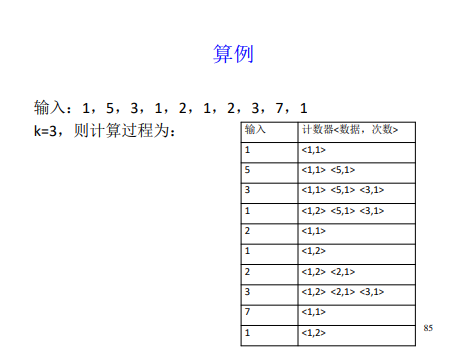
\includegraphics[scale=0.6]{Misra-Gries.png}
    \end{figure}
     
     \subsection{homework}
     
     \subsubsection{}证明二分查找是有序序列查找的最优算法
     \paragraph{Hint:}应为n个节点的二叉树(决策树)的高度为[logn] 所以必须经过logn才能达到叶子节点,O(logn)为查找的时间下界。故二分查找是最优算法。
     
     \subsubsection{}设A[1..n]是一个包含n个不同数的数组。如果在i<j的情况下有A[i]>A[j],则(i,j)为A中的一个逆序对。\\
     1)若A={2,3,8,6,1},列出其中所有的逆序对;\\
     2)若数组元素取自集合{1,2,…,n},那么怎样的数组含有最多的逆序对?它包含多少个逆序对?\\
     3)求任意数组A中逆序对的数目,并证明算法的时间复杂性为$\Omega (nlogn)$
     \paragraph{Hint:}1)(2,1);(3,1)\\
     2) n,n-1,...,1,$\frac{n(n-1)}{2}$对\\
     3)归并排序,在归并中计数


     \subsubsection{}有n个数存放在两个有序数组中,如何找到这n个数的第k小的数
     \paragraph{Hint:}\textbf{1.归并排序}O(k);\\
     \textbf{2.二分法}假设A 和B 的元素个数都大于$\frac{k}{2}$,比较A[k/2]和B[k/2],如果A[k/2]>B[k/2],那么第k个元素肯定在A序列前k/2个元素中或者在B序列k/2以后的元素中。所以删除B序列前k/2个元素,k:=k/2。反之若A[k/2]<B[k/2],删除A序列前k/2个元素,k:=k/2。递归,若相等则返回。\\
     若其中有一个序列的元素不足k/2,假设为m(m<k/2),则取第m个元素,另一个取第k-m个元素。\\
     时间复杂度为O(log k)
     
     \subsubsection{}如何修改KMP算法,使之能够获得字符串B在字符串A中出现的次数
     \paragraph{Hint:}匹配成功后截去前面的序列,进行递归。
     
      \subsubsection{}序列T和P的最长公共子序列(LCS)L定义为T和P的共同子序列中最长的一个,而最短公共超序列(SCS)S定义为所有以T和P为子序列的序列中最短的一个。设计高效算法求序列T和P的LCS和SCS的长度。
     \paragraph{Hint:}
     
     \subsubsection{}设计高效算法求序列中出现次数大于n/4的所有元素。
     \paragraph{Hint:}Misra-Gries.png算法调用最多三次,每次删去成功了的。
     
     \subsubsection{}对于任意给定的4个1-10之间的整数(可以相同),判断是否可以通过整数四则运算得到24。
     \paragraph{Hint:}后缀式遍历。
     
     \subsubsection{}对玻璃瓶做强度测试,设地面高度为0,从0往上有刻度1到n,相邻两个刻度间距离都相等,如果一个玻璃瓶从刻度i落到地面没有破碎,而在高度i+1处落到地面时碎了,则此类玻璃瓶的强度为i。1)若只有一个样品供测试,如何得到该类玻璃瓶的强度;2)如果样品数量充足,如何用尽量少的测试次数得到强度;3)如果有两个样品,如何用尽量少的测试次数得到强度
     \paragraph{Hint:}1)顺序查找2)二分查找\\
     3)将刻度分为$\sqrt{n}$组,每组包含$\sqrt{n}$个刻度先用顺序查找查找每个组的最大刻度,从而可以确定是在哪个组,再用第二个瓶子在这个组内进行顺序查找,测试的次数$O(\sqrt{n})$
     
     \subsubsection{}有一个有$2^k*2^k$个格子的正方形棋盘,以及可以覆盖3个格子的L型条块,如何用这些L型条块覆盖棋盘上$2^k*2^k-1$个格子,条块之间不能相互覆盖,也不能伸出棋盘。
     \paragraph{Hint:}数学归纳法,假设k-1时成立,空出最右下角的一格,将四个相同的2*2放置,左下角逆时针旋转90°,右上角顺时针旋转90°,将L型纸片放在那个位置,此时满足k\\
     
     \subsubsection{}有$n=2^k$位选手参加一项单循环比赛,即每位选手都要与其他n-1位选手比赛,且在n-1天内每人每天进行一场比赛,\\
     1)设计算法以得到赛程安排;\\
     2)若比赛结果存放在一矩阵中,针对该矩阵设计O(nlogn)的算法,为各个选手赋予次序P1,P2,…,Pn,使得P1打败P2,P2打败P3,依此类推。
     
     \paragraph{Hint:}1)利用分治法,把选手分成2组,每组组内进行循环赛,需n/2-1天,然后在n/2天内进行组间比赛\\
     2)与归并排序、快速排序类似\\

     
      \subsubsection{}每个螺母需要一个螺栓配套使用,现有n个不同尺寸的螺母和相应的n个螺栓,如何快速地为为每一个螺母找到对应的螺栓?只允许将一个螺母与一个螺栓进行匹配尝试,从而知道相互之间的大小关系,不能够比较两个螺母的大小,也不能比较两个螺栓的大小
     \paragraph{Hint:}用一个螺母和所有螺栓进行对比,从而得到较小的螺栓集合S和较大的螺栓集合L,以及一个配套的螺栓,再利用此螺栓与所有螺母配对,可以将螺母分入集合S和L,从而得到两个小规模问题。\\
     T(n)=Σ(T(s)+T(n-1-s))/n+(2n-1)与快速排序类似\\
     
     \section{图算法}
     \subsection{PPT}
     
     \subsubsection{}深度优先搜索(DFS)
     \paragraph{Hint:}对于一个用邻接表表示的无向图,遍历是从任意一个顶点r开始,它称之为DFS的根,这个根被标记为被访问过。然后,从与r连接的顶点中任意挑一个(未被标记过的)顶点r1,再从r1开始(递归)执行DFS。当到达一个顶点v,它的所有连接顶点都已经被标记过了,则递归停止。如果当对r1进行DFS终止后,所有与r连接的顶点都已经被标记过了,则对r进行的DFS终止。否则,在与r连接的顶点中任选一个未被标记过的顶点r2,从r2开始进行DFS,等等。
    
\lstset{language=C}
    \begin{lstlisting}
    Algorithm Depth_First_Search(G,v);
    Input: G=(V,E) (an undirected connected graph)
    v (a vertex of G)
    Output: depends on the application
    begin
        mark v;
        {preWORK depends on the application of DFS}
        
        perform preWORK on v; 
        for all edges (v,w) do
            if w is unmarked then Depth_First_Search(G,w);
            perform postWORK for (v,w);
            {postWORK depends on the application of DFS; 
            it is sometimes performed only on edges 
            leading to newly marked vertices}
      \end{lstlisting}
     
     \subsubsection{}给定一个有向图G=(V,E),确定它是否含有一个(有向)闭链。
     \paragraph{Hint:}引理7.4:令G=(V,E)是一个有向图,且令T是G的一个DFS树。则当且仅当G含有一个(相对于T的)\textbf{后退边}时,G含有一个有向闭链。\\
     故用DFS解决。\\
     注:有向图进行DFS后有四种类型的边:树边,后退边,前向边,和交叉边。前三类边连接两个顶点,其中一个是另一个在树中的后代:树边把树中的parents连接到children,后退边把后代连接到祖先,而前向边把祖先连接到后代。只有交叉边连接在树中无“关联”的两个顶点,且必须“从右到左”交叉。
     
     \lstset{language=C}
    \begin{lstlisting}
Algorithm Find_a_Cycle(G);
Input: G=(V,E) (a directed graph)
Output: Find_a_Cycle (true if G contains a cycle and false otherwise)
Use DFS, starting from an arbitrary vertex, 
with the following preWORK and postWORK:

preWORK:
    v.on_the_path:=true;
    //x.on_the_path is true if x 
    //is on the path from the root to the current vertex}
    //initially x.on_the_path=false for all vertices, 
    //and Find_a_Cycle is false
postWORK:
    if w.on_the_path then Find_a_Cycle:=true; halt;
    if w is the last vertex on v’s list then v.on_the_path:=false

    
    
      \end{lstlisting}

     \subsubsection{}广度优先搜索(BFS)
     \paragraph{Hint:}从顶点v开始,首先访问v全部的儿子,接着访问全部的“孙子”,依次类推。如果顶点w是通过BFS被标记的第k个顶点,则其具有的BFS数为k。通过只保留导向新访问顶点的边,可以构造一个BFS树。\\
          \lstset{language=C}
    \begin{lstlisting}
Algorithm Breadth_First_Search(G,v);
Input: G=(V,E) (an undirected connected graph), and v (a vertex of G)
Output: depends on the application
begin
    mark v;
    put v in a queue {First In First Out};
    while the queue is not empty do
        remove the first vertex w from the queue;
        perform preWORK on w; {depends on the application}
        for all edges (w,x) such that x is unmarked do
            mark x, add (w,x) to the tree T, put x in the queue
end

      \end{lstlisting}
      
      
           
          
     \subsubsection{}(拓扑排序)问题:给定一个有向非循环图G=(V,E),它有n个顶点,把顶点按照1到n做标记,满足,若v被标记为k,则通过有向路径从v出发可以到达的所有顶点的标记>k。
     \paragraph{Hint:}
只有一个顶点的基础情形是平凡的。\\
归纳假设:已知如何根据条件对顶点数<n的有向非循环图做标记。\\
引理 7.8:一个有向非循环图总有一个入度为0的顶点。找到一个入度为0的顶点,把它标记为1,并删除与它相连的边,再对剩下的图进行标记,

  \lstset{language=C}
    \begin{lstlisting}
    Algorithm Topological_Sorting(G);
Input: G=(V,E) (a directed acyclic graph)
Output: The Label field indicates a topological sorting of G
begin
    Initialize v.Indegree for all vertices; {eg., by DFS}
    G_label:=0;
    for i:=1 to n do
        if v[i].Indegree=0 then put v[i] in Queue;
    repeat
        remove vertex v from Queue;
        G_label:=G_label+1;
        v.label:=G_label;
        for all edges (v,w) do
            w.Indegree:=w.Indegree-1;
            if w.Indegree=0 then put w in Queue;
    until Queue is empty
end

  \end{lstlisting}
  
     复杂性:对变量Indegree进行初始化需要O(|V|+|E|)时间,找到一个入度为0的顶点需要常数式时间(访问一个队列)。当v从队列中删除时每一条边(v,w)被访问一次,因此,变量需要被更新的次数正好等于图中边的数目。从而\textbf{算法的运行时间是O(|V|+|E|)},这对于输入规模是线性的。
     
     
     \subsubsection{}(单源最短路径)给定有向图G=(V,E)及一个顶点v,寻找到从v出发到达G中其他各顶点的最短路径。
     \paragraph{Hint:}若是非循环则用拓扑排序O(|V|+|E|),循环图则用Dijkstra算法O((|E|+|V|)log|V|)。
    
     \subsubsection{}最小代价生成树MCST(给定一个无向连通图G=(V,E),找出G的具有最小代价的生成树T。)
     \paragraph{Hint:} 贪婪法,时间复杂度为O((|V|+|E|)log|V|)。
     
       
     \subsubsection{}(全部最短路径)给定一个(有向或无向)加权图G=(V,E),其权值为非负数,要找到所有顶点对之间的最小长度路径。
     \paragraph{Hint:}如果图是相对稀疏的,通过使用单源算法|V|次较好,其运行时间是O(|E||V|log|V|)。\\
     但是对于稠密图,用Floyd算法$O(|V|^3)$
     
     \subsubsection{}(传递闭包)给定一个有向图G=(V,E),G的传递闭包C=(V,F)是一个有向图,满足当且仅当在G中存在一条从v到w的路径,则在C中存在一条边(v,w)。问题:给定一个有向图G=(V,E),找到它的传递闭包。
     \paragraph{Hint:}构造G'=(V,E')是一个完全有向图(即所有的顶点之间都有双向连接)。对E'中每一条边e,如果$e\in E$则赋予长度值0,否则为1。然后转为求全部节点最短路径问题(若为0则连通)。
     
     \subsubsection{}(双连通分支)双连通:一个无向图是双连通的,如果从每一顶点到另一顶点至少存在两条不相交的路径。一个无向图被称为k连通的,如果在每两个顶点之间至少存在k条不相交的路径。一个图不是双连通的当且仅当存在一个顶点,把它删除后即可分离该图。这样的一个顶点被称之为关节点。\\
     双连通分支:一个双连通分支是一个\textbf{边}的最大子集,其导出子图是双连通的(即不存在一个更大的把它包含在内的子图,其导出子图是双连通图)。每一条边仅属于一个双连通分支。\\
     问题:如何划分双连通分支。
     

     \paragraph{Hint:}把每一个双连通分支看成一个节点,按照DFS构造这棵树,对于双连通树,添加边,如果边来自不同分支在树中产生一个闭链,所有节点合并成一个分支。如果这条边链接关节点,则这条边本身就是一个双连通分支(要求是简单图),如果这条边在一个分支中,则忽略不计。\textbf{未写完}
     
     算法的运行时间是O(|V|+|E|)。需要的空间也是O(|V|+|E|).
     
     \subsubsection{}(强连通分支)
     \paragraph{Hint:}
     
     
      \subsubsection{}问题:给定一个连通无向图G=(V,E),判定它是否存在一个偶数长度的闭链。
     \paragraph{Hint:}一个闭链必定包含在一个双连通分支中。因此,可以先把图划分成双连通分支,然后分别考察每一个分支。\\
定理 7.13:边数多于一的,并且不只有一个奇数长度闭链的双连通图,必然有一个长度为偶数的闭链。\\

     
    \subsubsection{}问题:给定一个有向图G=(V,E),判定是否包含一个奇数长度的(有向)闭链。
     \paragraph{Hint:}一个闭链必定包含在一个强连通分支中,所以可以同样假定图是强连通的。\\
从任一顶点r开始执行DFS,并且对顶点做偶数或者奇数的标记。把r标记为偶数,然后对于每一条边(v,w),对v和w做各自相反的标记。由于r可以从任意顶点到达,则有一个奇数长度闭链当且仅当试图对某个顶点进行标记时发现它已经被做过相反的标记了。\\
     
     
      \subsubsection{}(匹配)给定一个无向图G=(V,E),匹配是边的一个集合,其中任意两条边没有公共的顶点。\\
一个与匹配中任何边都不相关联的顶点称为无匹配的,或称这个顶点不属于该匹配。\\
一个完美匹配是所有顶点都有匹配的匹配。\\
一个最大匹配是具有最大边数的匹配。\\
一个极大匹配是不可能再增加边数的匹配。\\
问题:令G=(V,E)是一个无向图,其|V|=2n并且每个顶点的度至少为n。寻找完美匹配
     \paragraph{Hint:}在图G中考虑一个有m条边的匹配M,m<n。先检查所有不在M中的的边,看是否其中的一条可以加入到M中。如果找到这样的一条边则完成。否则,M就是个极大匹配。由于M不是完美的,至少有两个不相邻的顶点v1和v2不属于M。这两个顶点至少有2n条各不相同的边指向被M覆盖的顶点,如果不然的话,则有一条边可以加入M中。由于M的边数<n且从v1和v2出发有2n条边与它相连,所以至少有一条属于M的边,设为(u1,u2),与来自v1和v2的三条边相连。不失一般性,假定这三条边是(u1,v1),(u1,v2)和(u2,v1),通过从M中删除边(u1,u2),并增加两条边(u1,v2)和(u2,v1),可得到一个更大的匹配。
   \begin{figure}[h]
 	\centering
 	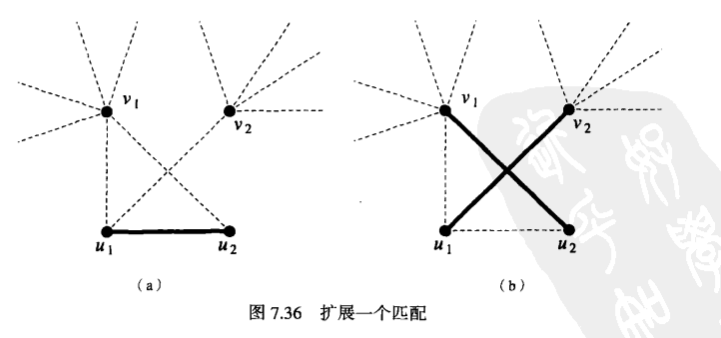
\includegraphics[scale=0.6]{Max.png}
    \end{figure}
    
     
    \subsubsection{}令G=(V,E,U)是一个偶图,其中V和U是两个不相交的顶点集合,E是连接V和U之间顶点的边集合。问题:在偶图中找到一个最大匹配。
     \paragraph{Hint:}
     交叉路径:对于一个给定匹配M,一个交互路径P是一个从V中顶点v出发到达U中顶点u的路径,而v和u都没有在M中被匹配,且P中的边交互出现在E-M和M中。这个交互路径可以用来改进匹配,用P中不在M里的边来替换M里的边,则得到另一个多一条边数的匹配。\\
     交互路径定理:一个匹配是最大的,当且仅当它不存在交互路径。\\
     先得出一个极大路径,再搜索交叉路径进行替换,而在任何匹配中至多有n/2条边(n是顶点数),所以迭代次数至多为n/2。\\
     
搜索的复杂性是O(|V|+|E|),因此算法的复杂性是O(|V|(|V|+|E|))。\\
改进:在G'中从V中未被匹配顶点集开始执行BFS,逐层进行,一直到在U中找到未被匹配的顶点。然后,通过BFS导出的图,抽取出G/中顶点不相交路径的极大集合(这就是G中的交互路径)。找到任何一个路径后,删除它的顶点,然后找另一条路径,再删除顶点,一直下去。为了在搜索中最大化匹配的边数(每一个顶点不相交路径为匹配增加一条边),选择一个极大集合。最后,利用交互路径集合修改匹配。这个过程一直重复到找不到更多的交互路径。\\
复杂性:改进过的算法在最坏情形的迭代次数是$O(\sqrt{n})$

       
     \subsubsection{}(哈密顿回路)哈密顿回路:一个简单回路,其包含V中每个顶点一次且仅一次。\\
     在非常稠密的图中找哈密顿回路,问题:给定连通无向图G=(V,E),其顶点数$n \geq 3$,且每一对非邻接顶点v和w满足$d(v)+d(w)\geq n$,在G中寻找一个哈密尔顿回路。(由Ore定理,图G存在哈密尔顿回路)

     \paragraph{Hint:}(反向归纳法)归纳假设:已知如何在满足给定条件,且边数$\geq m$的图中找到一个哈密尔顿回路。
     
     由归纳假设在G'中找到哈密尔顿回路x1,x2,…,xn,x1。如果边(v,w)不包含在这个回路中则完成,否则设v=x1且w=xn。\\
     由G中给定的条件$d(v)+d(w)\geq n$,G中所有从v和w发出的边至少有n条。\\
     在回路中存在两个邻接顶点$x_i$和$x_{i+1}$,其中v与$x_{i+1}$连接而w与$x_{i}$连接。利用边(v,$x_{i+1}$)和(w,$x_{i}$)可以得到一个不经过(v,w)的新哈密尔顿回路v(=$x_1$),$x_{i+1}$,$x_{i}$,…,w(=xn),$x_{i}$,$x_{i-1}$,…,v

     算法的时间复杂度为$O(n^2)$
     
     
     \subsection{homework}
     
     \subsubsection{} G=(V,E)是一个无向图,每个顶点的度数都为偶数,设计线性时间算法,给G中每条边一个方向,使每个顶点的入度等于出度。(请先简单说明算法思想,再给出伪代码,然后证明其时间复杂性符合要求)
     \paragraph{Hint:}即G为欧拉图,求欧拉回路\\
     
     \subsubsection{}连连看游戏中用户可以把两个相同的图用线连到一起,如果连线拐的弯小于等于两个则表示可以消去。设计算法,判断指定的两个图形能否消去。如果是求两个图形间的最少转弯次数呢?
     \paragraph{Hint:}1)DFS\\
        2)BFS:设两个图形为A(x1,y1)和B(x2,y2)\\
        i)求A可直接到达的格子,记为S0(有些为空格,最多4个图形),若$B\in S0$结束。\\
        ii)对S0中的空格,分别找的它们可直接到达的格子,记为S1:$S0 \in S1$,令S1’=S1-S0,即S1’中的格子和A可通过一次转弯到达,若$B \in S2’$结束。\\
        iii)对S1’中的空格,分别找到它们可直接到达的格子,记为S2,S2’=S2-S1-S0=S2-S1’-S0。即S2’中的格子和A可通过的1次转弯到达,若B∈S2’结束,否则无解。\\
        3)检查经过A,B的两条水平线之间是否有可行的垂直线,以及经过A,B的两条直线之间是否有可行的水平线。此算法速度快,推广性差。\\
        4)若求最少转弯次数,可用DFS,且在搜索时优先沿用上一次的方向。\\

     
     
     \subsubsection{}证明任意连通无向图中必然存在一个点,删除该点不影响图的连通性。用线性时间找到这个点
     \paragraph{Hint:}证明:进行双连通分支的划分,如果存在一个双连通分支不是单边的,删除这个双连通分支的一个节点不影响连通性。如果没有,那么这个图是一个树,删除叶子节点即可。\\
     线性时间找到用DFS,该点为DFS的叶子\\
     
     \subsubsection{}设G是有向非循环图,其所有路径最多含k条边,设计线性时间算法,将所有顶点分为k+1组,每一组中任意两个点之间不存在路径
     \paragraph{Hint:}拓扑排序,一次性移除队列中所有度数为0的点并归为一组
     
     \subsubsection{}给定连通无向图G,以及3条边a,b,c,在线性时间内判断G中是否存在一个包含a和b但不含c的闭链。
     \paragraph{Hint:}将c去掉,检查所有双连通分支划分,检查a和b是否在同一个分支内。
     
     \subsubsection{}设计线性时间算法求树的最大匹配
     \paragraph{Hint:}算法:将树视为根树,取任意的叶子v,将其与父节点w匹配,删除v和w(v的所有兄弟将不会被连接)得到小规模的树,可以通过归纳解决余下问题。\\
     证明(v,w)属于最大匹配:如果边(v,w)不在最大匹配中,那么v没有被匹配,则点w必然属于该匹配,即存在边(u,w)属于匹配,用(v,w)替换(u,w)。
     
     \subsubsection{}无向图G的\textbf{顶点覆盖}是指顶点集合U,G中每条边都至少有一个顶点在此集合中。设计线性时间算法为\textbf{树}寻找一个顶点覆盖,并且使该点集的规模尽量小。
     \paragraph{Hint:}从叶子开始归纳,叶子所在的边要被覆盖则选择叶子的父节点加入U,删除相关的边得到最小规模的树。 (其实和上述算法相似)
     
     \section{数学归纳法,树和机器学习}
     \subsection{PPT}
     应该不考
     
     \section{几何算法}
     \subsection{PPT}
     
     \subsubsection{}(判定点是否在多边形内部)问题:给定简单多边形P和点q,判定该点是在多边形内部,还是在多边形外部。

     \paragraph{Hint:}\textbf{一般说来},点在多边形的内部当且仅当由多边形外部任意一点到此点的连线与多边形的交点个数是奇数。\\
     \textbf{存在特例!} 比如经过了多边形的顶点。
       \lstset{language=C}
    \begin{lstlisting}
    Algorithm Point_in_Polygon_2(P,q)
    Input: P (a simple polygon with vertices p1,p2,...,pn
    and edges e1,e2,...,en), q =(x0,y0)(a point)
    Output: Inside (a Boolean variable that is set to true if q is inside P and false otherwise)
    begin
        count:=0;
        for all edges ei of the polygon do
            if the line x=x0 intersects ei then
                Let yi be the y coordinates of 
                the intersection between the line x=x0 and ei;
            if yi<y0 then increment count
        if count is odd then Inside:=true
        else Inside:=false;
    end

    \end{lstlisting}
    
算法复杂度:计算平面中两线段的交点需要花费常数时间,该算法计算n次这样
的交点(此处n指多边形的大小),而执行其他操作需要花费常数时间。因此,
该算法总共运行时间是O(n)。\textbf{需要添加对特例的判断}
    
     \subsubsection{}(构造简单多边形)问题:给定平面中n个点,将它们连接起来形成一条简单的封闭路径。
     \paragraph{Hint:}\textbf{圆心旋转}:存在特例,在$p_i,p_{i+1}$之间角度过180度时,这个可能就会出现交叉边\\
     可以考虑圆心选在任意三个节点的中心点上,也可以选择最大x坐标的点上(多个则选最小y坐标)(\textbf{仍然有特例:}可能会有重合的边)。
            \lstset{language=C}
    \begin{lstlisting}
    
    Algorithm Simple_polygon(p1,p2,...,pn)
    Input: p1, p2, ..., pn(points in the plane)
    Output: P (a simple polygon whose vertices are p1, p2, ..., pnin some order)
    begin
        choose the point with the largest x coordinate (and smallest y
        coordinate if there are several points with the same largest x
        coordinate) as p1
        for i:=2 to n do
            compute the angle ai between the line -p1-pi- and the x axis;
        Sort the points according to the angle a2,...,an;
        P is the polygon defined by the list of the points in sorted order
    end 
    
   \end{lstlisting}
     
     
     如何计算角度?tan \\
     角度相同时如何计算距离? $(xi-x0)^2+(yi-y0)^2$\\
     
     \subsubsection{}\textbf{凸包}:点集的凸包为包围所有点的最小凸多边形。\\
问题:计算平面中给定n个点的凸包。\\
凸包的顶点均来自集合中的点,如果一点是凸包的顶点,则称
其属于凸包。

     \paragraph{Hint:}\textbf{(1)直接法:}1.得到n-1个点的凸包。2.第n个点若在凸包内则不变,在凸包外则延拓。\\
     选取具有最大x坐标值的点(如果多个点有着相同的最大的x坐标值,则选取其中y坐标最小的点),将这个点标记为q,q必为凸包的顶点。现在考虑如何修改(延拓)凸包使之包括q。\\
     
     算法:首先,寻找原先属于旧凸包并且现在位于新凸包内部的点并将它们删除;接着,在两个现有顶点之间将这个新点作为新顶点插入。\\
    
    寻找被替代的点:\\
    \textbf{支撑线}:是指和多边形恰好只有一个交点的直线,即多边形全部位于支撑线的一侧。\\
    被删除的点是q最大最小支撑线中的点之间的节点。
                \lstset{language=C}
    \begin{lstlisting}
    convex(n)
    {
    if n=3 return 三角形
    找出x坐标最大的点,设为pn
    P=conver(n-1)为前n-1个点构成的凸包
    求pn到P所有顶点的角度,求出最大和最小值
    修正P的顶点列表得到新凸包P’
    return P’
    }
    
   \end{lstlisting}
   算法复杂度:对于每个点,需要计算其和先前诸点的角度,寻找其中最大和最小角度,并从顶点列表中添加和删除点,所以处理第k个点的时间为O(k)。由递推关系T(n)=T(n-1)+O(n)得到该算法的运行时间是O($n^2$)。 
   
   \textbf{(2)Gift Wrapping:}从一个极端点(它必须在这个凸包上)出发,通过寻找支撑线的方法发现它在凸包上的相邻顶点,然后以相同方式从这些相邻顶点出发继续该过程。\\
   算法复杂度:为了将第k个点添加进凸包,必须在n-k条直线中寻找最大和最小角度。所以算法的运行时间是$O(n^2)$,这并不比先前的延拓算法优越。
   
   
   \textbf{Graham扫描算法:}先用Simple Polygon算法排序,我们可以在前k个点中找到一条凸路径,在对凸路径进行处理,考察各个角度,如果小于180度,则属于凸包,否则删除这个点连接边上两个点,但是修改后的路径不一定是凸的。必须继续检查路径的最后两条边,直至找到两条所成角度小于180度的边,这时路径为凸。
      \begin{figure}[h]
 	\centering
 	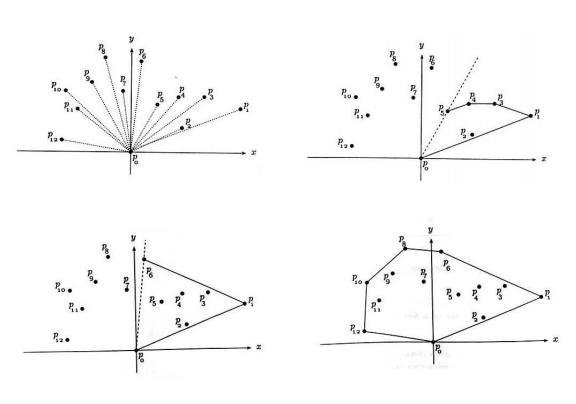
\includegraphics[scale=0.6]{Graham.png}
    \end{figure}
    
   算法复杂度:该算法的复杂度主要由排序所决定,所有其他步
骤仅需要O(n)时间,总共运行时间为O(nlogn)。
     \subsubsection{}(最近点对)问题:给定平面中n个点,寻找相距最近的点对。

     \paragraph{Hint:}直接方法:检查所有的点对,然后取最小值。该方法需要n(n1)/2次距离计算以及n(n-1)/2-1次比较。\\
     \\
     使用归纳法的直接解法:先去除一个点,然后解决n-1个点的问题,最后再考虑这个额外点。$O(n^2)$\\
    \\
    分治法:将P划分成大小相等的两个子集(P1和P2)垂直分。假设直到两个子集中的最小距离d,则考虑分割线左右两边d范围内的点,并且对于每个点只要考虑y坐标相距d的对面的点。\\
      
    \begin{figure}[h]
 	\centering
 	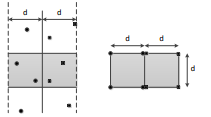
\includegraphics[scale=0.6]{nearestpair.png}
    \end{figure}
     
    
    算法复杂度:根据x坐标排序要花费O(nlogn)步,但只需进行一
次。解决两个规模为n/2的子问题后,消除带状区域外的点可以
在O(n)步内完成,根据y坐标排序需要花费O(nlogn)步。最后,
扫描带状区域中的每个点,并将它依次和常数多个相邻点比较,
需要花费O(n)步。因此有T(n)=2T(n/2)+O(nlogn),T(2)=1,该递
归关系的解为$T(n)=O(nlog^{2}n)$。\\
\textbf{改进为O(nlogn)的算法}原因:在组合步骤中花费O(nlogn)时间对y坐标排序\\
归纳假设:给定平面中<n个点的集合,知道怎样找到最近距离以及怎样输出根据y坐标排序后的点集合。\\
不必在每一次组合解时都重新排序,只需要归并即可。递归关系变成T(n)=2T(n/2)+O(n),T(2)=1,从而可得T(n)=O(nlogn)。
     
     \subsubsection{}(水平线段和垂直线段的交点)问题:给定平面中n条水平线段和m条垂直线段,寻找它们之间所有的交点。

     \paragraph{Hint:}直接方法:每次求一条线段和所有其他线段进行比较,这样共需O(mn)次比较。\\
     扫描线算法:从左到右扫描,水平左端点入队,右端点出队,垂直线进行判断。最坏情况下仍然需要O(mn)次比较操作。则在入队的时候把水平线的y坐标从小到大入队,扫描到垂直线的时候直接用二分查找则可。
     
     \subsubsection{}线段交点的计算
     \paragraph{Hint:}扫描线算法
        \begin{figure}[h]
 	\centering
 	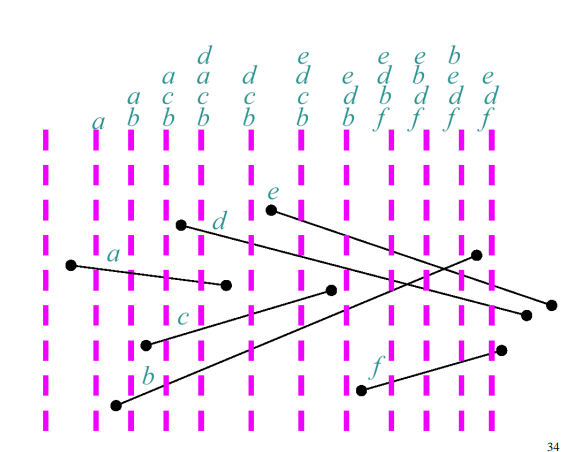
\includegraphics[scale=0.6]{scan.png}
    \end{figure}
    事件点:线段端点及线段交点,并按点的x坐标排序,依次在这些点进行处理:\\
    对于线段s的左端点:\\
    将线段s加入动态集合S中\\
    检查s在S中的相邻线段与s是否有交点\\
    对于线段s的右端点:\\
    从动态集合S中删除线段\\
    检查s在S中的相邻线段之间是否有交点\\
    对于线段s和t的交点:\\
    交换s和t的次序\\
    检查s,t和它们的相邻线段是否有交点 \\
     Time:\\
    O((2n+m)log(2n+m)) n是边数,m是交点个数
    
     \subsubsection{}定理(美术馆定理):对于任意的有n个顶点的简单多边
形,存在符合监控要求的保安集合,其中保安个数最多为$\lfloor n/3 \rfloor$
\textbf{简单多边形的三角划分}是指对多边形内部的分割,分割后得到的每个区域都是三角形,这些三角形的顶点为原多边形的顶点\\
三角划分可以视为求多边形最大的不相交对角线集合\\
问题:求多边形的三角划分。
     \paragraph{Hint:}两步走:\\
1)单调多边形的三角划分,O(n)\\
2)任意多边形划分为单调多边形,O(nlogn)\\
折线C被称为关于给定直线L是严格单调的是指对于任意与L垂直的直线与C最多只有一个交点\\
多边形P关于直线L单调是指其边界可以被分为两条折线,每条折线关于L都是单调的\\
\textbf{单调多边形的三角划分}:\\
假设多边形的顶点按照其x坐标递增的顺序排序\\
注意:这一假设不需要通过排序完成。提取上折线和下
折线,然后利用类似mergesort的方法对顶点进行合并,
时间复杂性为O(n)\\
三角划分的思想:通过增加对角线的方法将当前顶点左
侧部分三角化,并将得到的三角区域丢弃,在后面的
计算过程不再考虑\\

\textbf{一般多边形的单调划分}
为使用前述三角划分算法,首先需要将任意简单多边形
划分为单调多边形。这一过程也可通过扫描线算法实
现,算法将通过添加一系列互不相交的对角线将一般
多边形划分为一些单调多边形\\
转向点:假设沿着上折线或下折线从最左面的顶点走到
最右面的顶点,在此过程中如果在经过某个顶点时移
动的方向由向左变成向右,或者由向右变成向左,则
该顶点称为转向点,(内部角大于180度,并且
两条边要么都在该顶点左侧(此时该顶点称为合并
点),要么都在右侧(此时该顶点称为分离点))。\\
目标:通过添加对角线去除转向点\\
\\
扫描时如果遇到分离点v,则存在边ea在其上方,边eb在其下方\\
方法1:将v与ea或eb的左端点相连。但有可能v看不到这两个顶点。\\
方法2:找到ea和eb之间的顶点u,u和v相互之间能够看到\\
     
        \begin{figure}[h]
 	\centering
 	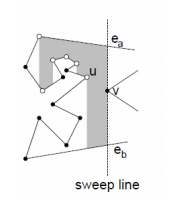
\includegraphics[scale=0.6]{dandiao.png}
    \end{figure}
     \textbf{未完成}
     
     \subsubsection{}给定n个半平面H ={h1, h2,…, hn},求交集\\
     \paragraph{Hint:}n个半平面的交集最多有n条边,分治法T(n)=2T(n/2)+S(n),如果S(n)=O(n),则总的计算时间为O(nlogn)。
     
     \subsubsection{} 如何在O(n)时间内计算两个凸多边形的交集 
\paragraph{Hint:}扫描线算法(扫描线与一个凸多边形至多两个交点,
因此扫描线状态表中最多只需记住4条边)。
在任意一点,下一个事件点最多只有8种可能性:4条与扫描线相交的边的右端点,这4条边的交点(最多4个)。因此对其操作都可以在常数时间内完成。
     
     \begin{figure}[h]
 	\centering
 	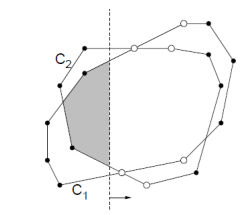
\includegraphics[scale=0.6]{tujiaoji.png}
    \end{figure}
    
      \subsubsection{}求Voronoi图(不赘述概念)
   \paragraph{Hint:}Fortune算法(扫描线算法添加海岸线(抛物线)(多条))
    \begin{figure}[h]
 	\centering
 	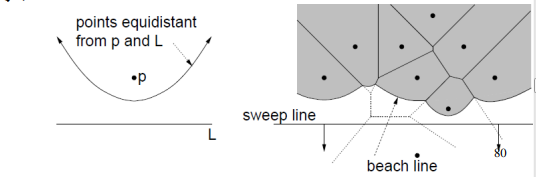
\includegraphics[scale=0.6]{Fortune.png}
    \end{figure}
    
    基点事件:扫描线经过一个新的基点时,一条新的抛物线会生成插入海岸线\\
顶点事件:当一条抛物线的长度缩减为0时,该抛物线消失,在这一点会生成一个新的Voronoi顶点\\
海岸线上的抛物线最多只有2n-1条,因为每个基点会生成
一条抛物线,并将已有的一条抛物线一分为二,从而
除了第一个基点外,每个基点都可以使抛物线总数增
加2
 \begin{figure}[h]
 	\centering
 	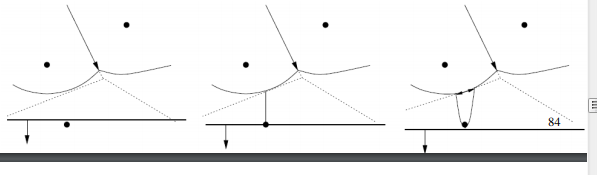
\includegraphics[scale=0.6]{jidianshijian.png}
    \end{figure}
    时间复杂性O(nlogn),空间复杂性O(n)

    
      \subsection{homework}
     
     \subsubsection{}设计算法判定平面上n个点是否在一条直线上
     \paragraph{Hint:}先给两个点连线求出来直线,遍历剩下的每个点是否在这条直线上就好。
     
     \subsubsection{}设P是包围在给定矩形R中的一个简单多边形,q为R中任意一点,设计高效算法寻找连接q和R外部一点的线段,使得该线段与P相交的边的数量最少
     \paragraph{Hint:}扫描线算法(旋转的扫描线),将多边形顶点按照它们与q的连线所成的角度进行排序,每次扫描过交点,如果两条线段的都在扫描线左侧,相交边+2,反之-2,若在两侧则不变。
     
     \subsubsection{}给定平面上一组点,已知每个点的坐标,求最远点对之间的距离,即点集的直径。(不得穷举,文献查阅,然后用自己的语言进行算法思想的描述,包括时间复杂性分析)
     \paragraph{Hint:}显然距离最远的两点一定位于一个点集的凸包上,这意味着可以采用时间复杂度为O(nlogn)的GRAHAM扫描算法进行预处理,而对于已有的凸包,则可以采用旋转凸包的方法求得其直径:对凸包的每条边,寻找与它距离最远的点,保存该点,该点至所选边两端点距离中的较大者,逆时针找到下一条边,同时从之前的点开始,逆时针寻找下一个点(避免重复探测),知道旋转一圈为止。\\
在最坏情况下,第二部分时间复杂度为O(n),故总时间复杂度为O(nlogn)。
     
     \subsubsection{}给定测度空间中位于同一平面的n个点,已知任意两点之间的距离dij,存储在矩阵D中,求这组点的直径。\\
该问题的直观解法就是把D扫描一遍,选择其中最大的元素即可。由于是在一个测度空间中,因此$d_{ij}$满足距离的基本要求,即非负性、对称性和三角不等式,我们就可以给出一种时间亚线性的近似算法。算法很简单,由原来确定性算法的检查整个矩阵改为只随机检查D的某一行,这样时间复杂性就由原来的$O(n^2)$减少为O(n),相对于输入规模$n^2$而言,这是一个时间亚线性的算法。那么时间代价减小的同时,证明解不会小于最优值的一半
     \paragraph{Hint:}假设我们随机抽取的定点为A,其中求得最长边为|AB|,若AB即为直径,则无需证明,若直径为|CD|,那么构造$\triangle ACD$,一定有|AD|+|AC|>|CD|,又有|AD|+|AC|<=2|AB|,所以2|AB|>|CD|,得证。
     
     \subsubsection{}在平面上给定一个有n个点的集合S,求S的极大点。极大点的定义:设p1=(x1,y1)和p2=(x2,y2)是平面上的两个点,如果$x1 \leq x2$并且$y1 \leq y2$,则称p2支配p1,记为p1 < p2 。点集S中的点p为极大点,意味着在S中找不到一个点q,$q \ne p$并且 p > q,即p不被S中其它点支配。
     \paragraph{Hint:}从右往左进行扫描,第一个点是极大点,接下来每次扫描得到的点,如果有纵坐标比当前极大点纵坐标大,即可更新极大点集以及当前极大点。
     
     \subsubsection{}对凸多边形,1)有多少种三角划分的方法?2)如何使对角线长度之和最小?
     \paragraph{Hint:}(1)
    \[ C(3) = 1 \]
    \[ C(4) = 2\]
     \[
        C(n) = \sum ^{n-2}_{k=3}C(k)C(n-k+1)+2C(n-1)
        \]     
  固定边(1,n),另一个点遍历2 到 n-1,用三角形分割多边形,其中2和n-1特殊处理。如果固定一个点用直线分割则为\[
            C(n)=\frac{n}{2(n-3)}\sum ^{n-1}_{k=3} C_{k}C_{n+2-k}
        \]
        
        2)设i<j,则由顶点i,i+1,...,j 构成的凸多边形添加对角线长度之和最小值为d[i,j],则$d[i,j]=min_{i+1\leq k \leq j+1} \{d[i,k]+d[k,j]+length(i,k)+length(k,j)\} , d[i,i+1]=0 $
        
     \subsubsection{}给定平面上n条线段,设计算法用O(nlogn)时间确定其中是否有两条线段相交。
     \paragraph{Hint:}课上的算法发现有交点后返回,因此事件点为2n
     
      \subsubsection{}用扫描线算法求解最近邻点对问题
     \paragraph{Hint:}从左到右扫描,事件点是每个点,扫描线状态记录与扫描线水平小于d的点,d为目前求得的最短距离,当扫描线遇到新的事件点时,计算与最近的常数个点的距离以判断是是否需要更新最短距离。
     
     \subsubsection{}有n种液体$S_1,S_2,…,S_n$,都含有A,B两种成分,含量分别为$\{ a_1,b_1 \},\{a_2,b_2 \},…,\{ a_n,b_n \},a_i+b_i<100 \% $。现欲利用这n种液体配制目标液体T,使之A和B的含量分别为x和y。设计算法判别能否成功配制,并给出算法时间复杂性。
     \paragraph{Hint:}转换为查看点是否在凸包内的问题,时间为O(nlogn)
     
         
     \subsubsection{}海报墙由n块宽度相同高度不同的木板组成,那么在此海报墙上能够张贴的最大海报面积是多少?设木板宽度为1,高度为$h_1,h_2,…,h_n$,海报必须整体都粘贴在墙上,并且不能斜贴。  
     \begin{figure}[h]
 	\centering
 	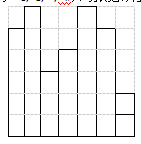
\includegraphics[scale=0.6]{poster.png}
    \end{figure}
    
     \paragraph{Hint:}基于第i块木板海报(高度为hi)最左边 最右边的位置为left[i]和right[i],则四边形的面积为(right[i]-left[i]-1)*hi\\
     
     从左到右依次考虑各块木板。\\
     第1块木板:左侧没有木板(或者说有一块高度为0的木板),所以left[1]=0,right[1]暂时无法计算。\\
     第2块木板:若 h1>h2, 则right[1]=2,从而求得第1号木板定义的最大四边形,并且第1块木板的信息不再需要,因为2号木板更低,以后的任意木板i不可能有left[j]=1,但right[2]暂时不能求。\\
     若h1=h2,则两块木板的最大四边形完全相同,1号木板的信息不再需要,可与h1>h2的情况一样处理。\\
     更进一步,对于第i块木板,若左侧有比自己高的木板,就能判断出以这些木板定义四边形会挡住自身定义的四边形,因此对这些木板求出最大四边形的面积后删除,那么,第i块木板左侧之比自己低的木板,从而求出left[i],可以利用栈存放未删除。\\
     
    \lstset{language=C}
    \begin{lstlisting} 
     1.初始化栈remain
     数组h存放木板高度,并且在最后增加一个0
     最大面积r=0
     for(i=1 ; i<= n+1 ; i++){
        while(remaining 非空 &&  h[remaining.top()]>=h[j]){
            j = remaining.pop()
            if(remaining 为空) width = i -1;
            else width = i-remaining.top()-1;
            r  = max(r, h[j]*width )
        }
        i 进 remaining
     }
     return r
     \end{lstlisting} 
     
     
     
     \subsubsection{}已知n个矩形,这些矩形的边都平行于坐标轴,\\
     1)识别出那些包含在另一个矩形中的矩形;\\
     2)求出这些矩形的交集;\\
     3)求出这些矩形能够覆盖的面积
     \paragraph{Hint:}1)按左边界排序,设前n-1个矩形已经处理完,扫描线状态记录与扫描线相交的矩形,并且按右边界从大到小排序,当遇到第n个矩形的左边界,检查其右边界是否比目前最大的右边界还大,如果是,则该矩形不会被前面的矩形包含,如果不是,则必然在x轴方向包含于某个已经扫描到的矩形,检查y方向是否包含,如果遇到右边界则该矩形可以去除。\\
     \\
2)扫描线:遇到左边界,求出已知最小左边界线段交集,遇到第一个右边界算法结束,若还有未发现的左边界,结果为空,否则结果矩形为最后一个左边界开始至第一个右边界,高度为最小左边界线段。\\
\\
3)每次遇到一条竖直边,计算这条边和前一条竖直边之间包含的所有矩形部分的横截面积。
     
     \subsubsection{}如何确定一个给定的多边形是简单多边形
     \paragraph{Hint:}判断多边形是否有非定点的交点即可。判断是否有交点与hw4第七题一样\\
     
     \subsubsection{}平面有两组点,如何证明存在直线可以将这两组点分开
     \paragraph{Hint:}求出凸包,用扫描线算法求出两个凸包的交集,若交集为空,则存在。\\

     
     \section{代数和数值算法}
     \subsection{PPT}
     
     \subsubsection{}计算$ \int ^{1}_{0} e^{-x^{2}}dx =0.747... $
     \paragraph{Hint:}Taylor展开再积分,$ \int^{1}_{0} e^{-x^{2}}dx = 1-\frac{1}{3}+\frac{1}{2!}*\frac{1}{5}-\frac{1}{3!}*\frac{1}{7}...$
     
     \subsubsection{}(大数吃小数)计算$ I_n = \frac{1}{e} \int ^{1}_{0} x^{n}e^{x}dx = 1 - nI_{n-1}$
     \paragraph{Hint:}根据$\frac{1}{e(N+1)}<I_{N}<\frac{1}{N+1}$得到估计值$I_{N}* = \frac{1}{2}(\frac{1}{e(N+1)}+\frac{1}{N+1})$再反推。
     
     \subsubsection{}求n的k次幂
     \paragraph{Hint:}类似于分治法,O(logk)
     
     \subsubsection{}最大公约数
     \paragraph{Hint:}辗转相除法,O(log(n+m))。
     如果k能同时整除m和n,那么它能整除后两者的差。如果n>m,那么GCD(n,m)=GCD(n-m,m)。
     
     \lstset{language=C}
    \begin{lstlisting} 
    Algorithm GCD(m,n)
    Input: m and n (two positive integers)
    Output: gcd (the gcd of m and n)
    begin
        a:=max(n,m);
        b:=min(n,m);
        r:=1;
        while r>0 do {r is the remainder}
            r:=a mod b;
            a:=b;
            b:=r;
        gcd:=a
    end

     \end{lstlisting} 
     
    \subsubsection{}多项式乘法:问题:给定n-1次多项式P和Q,计算乘积
     \paragraph{Hint:}直接方法:乘法和加法的运算量是$O(n^2)$\\
     分治算法:分为高低幂的P1,P2,Q1,Q2。运算量T(n)=4T(n/2)+O(n),T(1)=1,解是$O(n^2)$。
     设A=P1*Q1, B=P2*Q1, C=P1*Q2, D=P2*Q2,要计算$A+(B+C)x^{n/2}+Dx^{n}$,通过观察可以发现,不需要分别计算B和C,只需要得到它们的和即可!
     新递归关系为T(n)=3T(n/2)+O(n),从而可以推得$T(n)=O(n^{log_{2}3})=O(n^{1.59})$

     \subsubsection{}矩阵乘法
     \paragraph{Hint:}
     常规算法:$O(n^3)$\\
     Winograd算法:$O(n^3)$\\
     Strassen算法:$O(n^{2.81})$\\
     
     \subsubsection{}问题:计算两个n×n布尔矩阵的乘积
     \paragraph{Hint:}技巧1:环
技巧2:将k个操作数存储在一个大小为k的计算机字中。矩阵
乘法的常规算法由$n^2$个“行乘以列”的乘积(或内积)所组成,
假定k可整除n,因而可以将每个内积分解成n/k个k维布尔向
量的内积的总和。
思想一:\\
预先计算所有可能的k维布尔内积:由于其中涉及两个k维布尔
向量,所以共有$2^{2k}$种可能,可以在时间$O(k2^{2k})$内计算
$O(k2^{2k})$\\
例如例如,设$k= \lfloor log2n/2 \rfloor$,表的规模此时为O(n),构造该表本身需要O(nlogn)时间。建立表以后就可以在时间O(n/k)=O(n/logn)内计算n维布尔内积。因此,计算两布尔矩阵的乘积可以在时间$O(n…^{3}/logn)$以及额外空间O(n)内完成。也可以选取k为$\lfloor log_{2}n \rfloor$,此时表的
规模为$O(n^2)$,而矩阵乘法时间可以减半。\\
第二个思想:\\
将A的列、B的行划分成n/k个大小相等的组,记为$A_1,A_2...A_{n/k}$,B同理,设$C_i=A_i B_i$,其第j行是若干$B_i$行的布尔和(根据$A_i$的第j行)使用类似于前述算法中所使用的方法,即预先计算所有的可能性。
相比于先前的算法,该表包含n行而不是n比特;因此,存储空间需要$O(n^2)$。
综上,可以在时间$O(n^2)$内计算$C_i$。计算Bi行之和的各种可能组合需要$O(n2^k)$。\\
该算法总共的运行时间为$O(n^3/k+n^2 2^k/k)$。如果$k=log_2 n$,那么运行
时间即为$(n^3 /logn)$。\\

$O(n^3/log_2 n)$的方法:将表中的一行
加至C,通过使用相同的技巧——预先计算所有可能的加法
运算,可以在时间O(n/m)内完成加法运算。现在将$B_i$的
每一行分成n/m组,每组大小为m的元组\\


     \subsubsection{}矩阵链相乘
     \paragraph{Hint:}蛮力搜索法:尝试所有可能的计算次序,$\Omega (4^n / \sqrt{n})$\\
     转为背包问题解决时间$\Theta (n^3)$,空间$\Theta (n^2)$。
     
     
     \subsubsection{}假定在n个不同点对任意一个n-1次多项式P进行求值,并设n是2的幂
     \paragraph{Hint:}正向傅立叶变换,算法的复杂性为O(nlogn)。
     
     
     \subsubsection{}逆向傅立叶变换
     \paragraph{Hint:}
     
     
     \subsubsection{}非线性方程的数值解法
     \paragraph{Hint:}(1)二分法:收敛慢,对分次数\\
     (2)迭代法求根:f(x)=0 <==> x=g(x) 称为迭代函数\\
f(x)的根x* <==> g(x)的不动点x*,\\
从一个初值x0出发,计算x1 = g(x0), x2 =g(x1), …, xk+1 = g(xk), … \\
不一定能收敛\\
g(x) = x - f(x)/f'(x)
     (3)牛顿法:依赖于x0的选取\\
      \subsection{homework}
     
     \subsubsection{}求n!包含质因子p的数量,例如6!含有4个2,2个3和1个5,并给出算法的时间复杂性。
     \paragraph{Hint:}1)直接求2到n每个数有几个因子p,最后相加。O(nlogn)\\
     2) n! 有 $(n/p+n/p^{2}+n/p^{3}+……)$个因子p,O(logn) 质因数分解需要logn\\
     
     \subsubsection{}设Fibonacci数列的定义为:F(1)=1, F(2)=1, F(n)=F(n-1)+F(n-2) (n>2),证明每个大于2的整数n都可以写成至多logn个Fibonacci数之和,并设计算法对于给定的n寻找这样的表示方式
     \paragraph{Hint:}数学归纳法:\\
     若小于n的整数都满足要求,对于n找到不大于n的最大F数F(k),则F(k)大于n/2(否则F(k+1)<n).由归纳假设,n-F(k)可以写成最多log(n-F(k))个F数之和,由于n-F(k)<F(k),所以这些数都不会等于F(k),因此n最多可以用log(n-F(k))+1 < logn个F数之和。\\

     
     \subsubsection{}n个矩阵$M_1、M_2、...、M_n$相乘最多需要多少次乘法
     \paragraph{Hint:}与课上讲的完全相同,把min换成max\\
     

     
     \section{归约}
     \subsection{PPT}
     
     \subsubsection{}CSM问题:设两个长度为n的字符串A=a0a1...an-1及B=b0b1
...bn-1,判断B是否A的循环平移。
     \paragraph{Hint:}方法1:修改6.7节中介绍的Knuth-Morris-Pratt算法来解决CSM\\
方法2:寻找特定的文本T及特定的模式P使得在T中寻找P等同于判定B是否A的一个循环平移\\
答案:把T定义为AA(也就是A再连接它本身)。显然,B是A
的一个循环平移当且仅当B是AA的一个子串。既然已经知道如
何在线性时间内解决SM问题,那么同样有CSM问题的线性时
间算法。

     
     \subsubsection{}设S1,S2…,Sk是一组集合。不同代表集(System of Distinct
Representative ,SDR)是一个集合R={r1,r2,...rk},其中 $ri \in Si$。
由于R是集合,ri就必须是相异的,即R刚好包含每个集合的一个代表元素。给定一组集合未必能找到一个SDR\\
问题:给定一由有穷个有穷集合组成的组,找出该组的(任意
一个)SDR,或判断SDR是否存在。
     \paragraph{Hint:}设card(S)是S的元素个数。\\
     Hall定理:设$S_1,S_2,…,S_k$是一组集合,其存在SDR当且仅当下面
条件成立,$card(S_{i_1} \cup S_{i_2} \cup... \cup S_{i_m} ) \geq m $ 对$\{1,2,...,k\}$的任一个子集$\{i_1,i_2,...,i_m\}$,即任意m个集合的并必须至少包含m个不同的元素,对所有的$1\leq m \leq k$。\\
把它看成偶图匹配问题:设G=(V,U,E)是一个偶图,使得对每
个集合$S_i$均在V中存在一个顶点$v_i$,并且对所有可能的元素
(即对集合的并中的每个元素)在U中都有一个顶点$u_j$。则SDR就是G中规模为k
的匹配。
     
     \subsubsection{}序列比较:$A=a_1 a_2 …a_n$及$B=b_ 1 b_2 …b
     _ m$是两个字符串,要逐
字符地编辑A直到它变为B。允许插入、删除和替换三种编
辑方式,每个方式涉及一个字符,且已知这些方式的代价,
目标是使编辑的代价最小。

     \paragraph{Hint:}转为单源最短路径问题。\\
     把表看成一个有向图。表中每一项对应图的一个
顶点,这样每个顶点对应一个局部编辑。当v对应的局部编
辑能够经过一个以上编辑步骤到w对应的局部编辑时,则存
在一条边(v,w)。水平边对应插入,垂直边对应删除,而斜
边对应替换。除了对应相同字符的斜边(即无须替换)的
代价是0 ,其它每条边的代价是1。
     
     \subsubsection{}在无向图中寻找三角形
     \paragraph{Hint:}设A是G的邻接矩阵。因为G是无向的,所以A对称。算$A^2$即可。$A^2
[i,j]>0$当且仅当存在k使得A[i,k]和A[k,j]均为1,规约到布尔矩阵乘法问题。
     
     
     \subsubsection{}\textbf{线性规划:}
     线性规划问题可形式化阐述如下:在满足不等式约束,等式约束和非负约束的条件下使目标函数最大化。(标准形式,松弛变量)\\
     \textbf{网络流量问题}:G=(V,E)是一个有两个特殊顶点的有向图,一个是入度为0的
s(源点),一个是出度为0的t(汇点)。E中的每条边e赋予一个
正的权值c(e),称为e的容量,用来度量经过这条边的最大
流量,可为不存在的边赋予容量值0 。这样的一个图称为网
络。f(e)不能超过c(e),流入等于流出\\
     \paragraph{Hint:}可直接列出表达式归约为线性规划。存在容量约束,非负约束和流入等于流出等式约束。目标为总流量。

     \subsubsection{}\textbf{静态路由问题}:设G=(V,E)是无向图,表示一个通讯网络。假设网络中每个节
点有一个有限缓存,在一个单位时间内只能接收Bi条消息
(设所有消息的长度均相同)。再假设任一链路可以传输
的消息数目没有限制,每个节点均有无限的消息供应,问
题是在单位时间内每条边应该传送多少条消息才能使在网
络上的总消息数量最多。用图论表述,问题就是对边赋予
权重,连接节点Vi的边的权重≤Bi,而使所有权重的和最大
化。
     \paragraph{Hint:}和网络流量问题类似,目标为边的权重和,约束为接收和不能超过Bi和非负约束。
     
     
     \subsubsection{}\textbf{慈善家问题}:设有n个组织要向k个计算机系捐助,每个组织i在一年内都有
总捐助限度$s_i$,对部门j的捐助同样也有限度$a_{ij}$(对某些部门
$a_{ij}$可能是0)。一般来说$s_i$比$ \sum ^{k}_{j=1}a_{ij}$要小,因而每个组织都要做
一些抉择。此外,设每部门也有收受总金额的限制$t_
j$(虽然
这个约束不太现实,不过这是很有趣的)。目标是设计一
个算法使总捐助金额最大(不管公平与否)

     \paragraph{Hint:}一样的归约到线性规划
         
     \subsubsection{}\textbf{分配问题}对慈善家问题稍作更改:强调每个组织只能向一个部门捐助,
而每个部门也仅接收一个组织的捐助。

     \paragraph{Hint:}想比与之前添加一个变量xij,选择该边为1,不选择为0。目标函数为$\sum_{ij}a_{ij}x_{ij}$
     
     \subsubsection{}平凡下界:有一类下界被称为平凡下界,可以在不借助任何计算模型或者进行复杂计算的情况下
就能够得到。
     \paragraph{Hint:}对于一个没有排序的序列,为找出其中的最小数,必须检查序列中所有的数,因此在无序序
列中进行查找的任何算法必须花费$\Omega(n)$时间。
两个n*n矩阵相乘的任何算法都必须计算并输出恰好$n^2$个值,因此两个n*n矩阵相乘的任何算
法的时间复杂性为$\Omega(n^2)$。

     
     \subsubsection{}寻找简单多边形算法复杂度的下界
     \paragraph{Hint:}考虑用一个简单闭多边形连接平面上一系列点的问题,我们已
经知道如何用排序来解该问题,在某些假设下,这个问题
是不可能比排序来得更快。在最坏情况下需要$\Omega(nlogn)$的比较。
     
     \subsubsection{}基于比较的排序算法的下界
     \paragraph{Hint:}若各种输入情况等概率出现,则任何一个基于比较的排序算
法平均需要至少logn!-1次比较,其中n为待排序的数字个数


     \subsubsection{}关于矩阵的简单归约
 \paragraph{Hint:}定理10.3:如果有算法在O(T(n))时间内计算两个n×n的对称实
矩阵相乘 , 满 足 T(2n)=O(T(n)) , 那 么 同 样 有 算 法 在
O(T(n)+$n^2$
)时间内计算两个n×n的任意实矩阵相乘。\\
定理10.4:如果有算法在O(T(n))时间内计算n×n实矩阵的平方,
满足T(2n)=O(T(n)),那么同样有算法在O(T(n)+$n^2$
)时间内计
算两个n×n的任意实矩阵相乘。
    
      \subsection{homework}
      \subsubsection{}设有算法A能够在O(i)时间内计算一个i次多项式和一个1次多项式的乘积,算法B能够在O(ilogi)时间内计算两个i次多项式的乘积。现给定d个整数$n1,n2,…,nd$,设计算法求出满足$P(n1)=P(n2)=…=P(nd)=0$且最高次项系数为1的d次多项式P(x),并给出算法的时间复杂性
     \paragraph{Hint:}
     多项式的形式为(x-n1)(x-n2)...(x-nd)。\\
     两两合并用算法B,时间复杂度$O(dlog^{2}d)$。\\
     
     \subsubsection{}输入是由数轴上的区间所组成的集合,这些区间由它们的两个端点表示。设计O(nlogn)算法识别所有包含在集合中其它某个区间的区间。这个问题与二维平面极大点问题有什么关系例如输入:(1,3),(2,8),(4,6),(5,7),(7,9),则输出为(4,6)和(5,7)     
     \paragraph{Hint:}区间按左端点排序,依次处理,类似与极大点问题扫描右断点
     
     归约为极大点问题,对于区间I(j) = ( L(j), R(j) ),构造点( -L(j) , R(j))则一个区间包含于另一个区间等价于对应的点不是极大点。\\
     
     \subsubsection{}证明Graham算法是求凸包问题的一种最优算法
     \paragraph{Hint:}排序归约到凸包,待排序的数映射到单位圆上,所以凸包问题下界是O(nlogn).\\
     
     \subsubsection{}证明如果存在时间复杂度为O(T(n))的两个nn下三角矩阵的乘法,则存在时间复杂度为$O(T(n)+n^2)$的任意两个nn矩阵相乘的算法。
     \paragraph{Hint:}构造下三角矩阵[[ 0,0,0 ],[A,0,0],[A,A,0]]与[[ 0,0,0 ],[B,0,0],[B,B,0]]相乘得[[ 0,0,0],[0,0,0],[AB,0,0]]
     
     \subsubsection{}如果在序列$x_1,x_2,…,x_n$中,存在某个i使$x_i$是序列中的最小者,且序列$x_i,x_{i+1},…,x_n,x_1,…x_{i-1}$是递增的,则称序列$x_1,x_2,…,x_n$是循环序列。设计算法找出循环序列中最小元素的位置。为简单起见,假设该位置是唯一的。证明你的算法是最优的。
     \paragraph{Hint:}二分搜索,通过一次比较将序列长度减半,在序列中任取两个元素Xk,Xm,其中k<m。若Xk<Xm,i就不可能落在k<i<m中,因为Xi是序列中最小的数;反之,一定在k~m之间。时间复杂度为O(logn),决策树搞O(nlogn)\\
     
     \subsubsection{}(选做)现在有如下猜想需要验证:长得越胖的老鼠跑得越快。从算法设计的角度给出如何验证(或者否定)这一猜想,给出你的思路。
     \paragraph{Hint:}收集老鼠体重与速度的数据\\
     按重量升序排列,重量相同则按速度降序\\
     对序列寻找一个最长(速度)递增子序列\\
     (怀疑不全)\\
     
     \section{计算机不是万能的}
     \subsection{PPT}
     
     \subsubsection{}停机问题(Halting problem)
     \paragraph{Hint:}
     假如已经设计出了停机分析算法halt,虽然不知道halt的实现过程,但基于halt算
法设计如下算法strange
\lstset{language=C}
    \begin{lstlisting} 


算法 strange
输入:字符串p
1. result = halt(p,p)
2. if result == True {halt算法判定p(p)终止}
3.      while True //死循环
4.          pass
5.      end while
6. else {halt算法判定p(p)不终止}
7.      return
8. end if
     \end{lstlisting} 
那么运行strange(strange)的结果\\
若strange(strange)不终止,则strange(strange)终止;\\
若strange(strange)终止,则strange(strange)不终止。\\
     
     \subsubsection{}\textbf{顶点覆盖问题}:设G=(V,E)是一个无向图,G的顶点覆盖是一个顶点集合,满足G中
所有的边都至少和该集合中的一个顶点相关联。\\
问题:给定无向图G=(V,E)和一个整数k,判定G是否有包含$\leq$k个顶
点的顶点覆盖。
     \paragraph{Hint:}\textbf{顶点覆盖问题是NP完全的},将团问题归约到顶点覆盖问题。
     
     \subsubsection{}\textbf{支配集问题}设G=(V,E)是一个无向图,如果顶点集合D满足,G中的所有顶点要
么在D中要么与D中至少一个顶点相邻,则称D为支配集。\\
问题:给定无向图G=(V,E)和整数k,判定G中是否有一个包含$\leq$k个
顶点的支配集。

     \paragraph{Hint:}\textbf{支配集问题是NP完全的}将顶点覆盖问题归约到支配集问题
     
     
     \subsubsection{}\textbf{团问题:}给定无向图G=(V,E),G中的一个团C是G的一个子图,满足C中的任
何两个顶点均相邻,换句话说,团即完全子图。
问题:给定无向图G=(V,E)和整数k,判定G是否包含一个大小$\geq$k的
团。
     \paragraph{Hint:}\textbf{团问题是NP完全的。}将SAT问题归约到团问题
     
     \subsubsection{}\textbf{着色问题:}设G=(V,E)是无向图,G的有效着色是指对所有顶点的颜色指派,使
得每个顶点被指派一种颜色并且相邻顶点不被指派成相同颜色。
问题:给定无向图G=(V,E),判定G是否可以被3种颜色着色。
     \paragraph{Hint:}\textbf{着色问题是NP完全的。}将3SAT问题归约到3着色问题\\
     回溯法解决。\\
     
     
     \paragraph{归约是从一个已知NP完全问题的任意实例到问题Q,通常最容易犯的错
误是反方向进行归约}

     \subsubsection{}常见的NP完全问题
     \paragraph{Hint:}哈密尔顿问题:给出无向图G=(V,E),是否存在一条遍历每个顶点一次且仅一次的
路径?\\
旅行商问题:给出加权无向图G=(V,E),求出遍历每个顶点一次且仅一次的最短路
径\\
0-1背包问题:U={u1
, u2
,..., un
}是一个准备放入容量为C的背包中的n个物品的集合,
第i个物品ui具有体积si和价值vi,要求从这n个物品中挑选出一部分装入背包,
在不超过背包容量的前提下使背包中物品的价值最大。\\
装箱问题:给出大小为s1
, s2
, …, sn的n个物品,能否最多用k个容量为C的箱子将这
些物品装入?\\
\indent 分枝限界法解决(不停的求上下界)\\

集合覆盖问题:给定集合X以及X的子集族F,是否存在F中的k个子集,它们的并
集是X?\\
作业调度问题:有n个作业J1
, J2
, …, Jn,每项作业J
i的需要的机器运行时间为ti,那
么能否在时间T内利用m台机器完成所有n项作业?\\


    \subsubsection{}顶点覆盖问题的近似算法
  \paragraph{Hint:}求极大匹配,定理:与极大匹配M中的边相关联的所有顶点构成一个顶点覆
盖,并且其大小不超过最小顶点覆盖大小的2倍。\\
但寻找最小极大匹配(即有最少边个数的极大匹配)问题也是NP完全的


 \subsubsection{}一维箱柜包装问题:箱柜包装问题是指将不同大小物体打包到规定大小的箱柜中,并
且箱柜使用的数目要尽可能少。
\paragraph{Hint:}逆序排序后Firstfit算法.定理:Decreasing First Fit算法至多需要11/9OPT+4个箱柜。

 \subsubsection{}欧几里德旅行商问题:问题:C1
,C2
,...,Cn 是平面中的点集合,其对应于n个城市的位置;
试找到一条长度最短的哈密尔顿回路

\paragraph{Hint:}首先计算最小代价生成树(这里代价=距离),树的代价不会超过最佳TSP长度。考察由深度优先搜索遍历树(从任意顶点出发)所形成的环路,每条边恰好被遍历了两次,所以这个环路的代价是这棵最小生
成树代价的两倍,因而也不会超过最短TSP行程的两倍。\\
改进:高效转为欧拉图对这棵树添加足够多的边,使得所有节点的度均为偶数,这样就得到了一个欧拉图。由于TSP路径将由这个欧拉环路(会走一些
捷径)构成,因此要将额外添加的边的长度最小化\\
改进:问题:给定平面中的一棵树,希望添加一些边使之成为一个欧拉
图,并且要使添加边的总长最小。\\
定理11.12:改进后算法所生成的TSP行程,其长度至多为最短TSP
行程长度的1.5倍。\\



 \subsubsection{}需要判断RI 和 RII 的数据是否相同
\paragraph{Hint:} 随机算法:在$[2, n^2]$ 内随机选择素数p\\
RI计算得到整数s = Number(x) mod p,将s和p的二进制表示发送
给RII\\
收到s和p之后,RII 计算q = Number(y) mod p.\\
错误率最多为$(ln n^2)/n$ 


      \subsection{homework}
     \subsubsection{}计算机病毒判定问题:计算机病毒的特点是能够感染其它程序,并且具有一定的破坏性,证明我们无法在新品种病毒发作前发现新品种的病毒
     \paragraph{Hint:}因为他发作前没有办法判定他是否能够感染其他程序并且是否具有破坏性。
     
     \subsubsection{}证明求n的k次幂问题是P类问题
     \paragraph{Hint:}将求n的k次幂问题转换为求n的k/2次幂和n的k-k/2次幂问题。而求n的2次幂是一个P类问题且转换也是高效的。
     
     \subsubsection{}设计一个不确定性算法求解旅行商问题
     \paragraph{Hint:}对图中每条边而言,随机地决定是否保留。对所有保留的边,判断是否能够经过所有顶点且距离之和小于d
     
     
     
     \subsubsection{}设和 $\Pi'$ 和 $\Pi$
     是两个NP完全问题,证明或否定$\Pi' \propto _{poly} \Pi$
     \paragraph{Hint:}$\Pi$和$\Pi'$都是NP完全问题,则$\Pi$和$\Pi$’都在NP中,且所有NP中的问题都可以多项式规约到$\Pi$和$\Pi$’,所以也可以在多项式时间内规约到$\Pi$’。
     
     \subsubsection{}是否有可能在多项式时间内判断无向图G=(V,E)存在规模为5的团集?为什么?
     \paragraph{Hint:}可能,规模为5的子集为$O(n^5)$判定是否为完全图只需要常数时间。
     
     \subsubsection{}阅读2-sat问题的材料2SAT.pptx
     \paragraph{Hint:}
     
     \subsubsection{}已知顶点覆盖问题是NP完全的,那么如果所有顶点的度数都是偶数,能不能设计出多项式时间的确定性算法?
     \paragraph{Hint:}增加一个三角形,它的顶点的度数都为2,而任意图中度数为奇数的点为偶数个,将他们全都连在三角形的某个顶点上
     
      \subsubsection{}3-MAX-SAT问题是指对于给定的由m个子句构成的合取范式F,每个子句恰好有3个文字,如何对布尔变量$x_1,x_2,…,x_n$赋值,使得F中满足的子句尽可能多。证明3-MAX-SAT问题是NP完全问题
     \paragraph{Hint:}3-SAT是NP完全问题,所以3-MAX-SAT一定也是NP完全问题。
     
     \subsubsection{} N皇后问题是指如何在一个nn的国际象棋棋盘上放置n个皇后,使得这些皇后不会相互攻击,即这些皇后没有两个在同一行、同一列或同一条对角线上。用回溯法求解。
     \paragraph{Hint:}从第一行第一个开始放,确定了第一个以后,往第二行放,一直往下,直到填满或者出现矛盾,若出现矛盾则向上回溯,直到解决矛盾为止,若填满了则回溯到倒数第二个,改变它的位置,往下走继续重复上述过程,若倒数第二个没有其他位置可以放就继续回溯到第三个……以此类推。
     
     \subsubsection{}任务分配问题要求把n项任务分配给n个人,每个人完成每项任务的成本不同,要求分配总成本最小的最优分配方案。图示是一个任务分配的成本矩阵。用分支限界法求解
     \paragraph{Hint:}若任务一分配给a,那么最小代价为
     9+4+4+4=21\\
b 6+2+2+2=12\\
c 5+2+2+2=11 :\\
\indent\indent a 5+2+3+3=13\\
\indent \indent b 5+2+3+4=17\\
\indent \indent	d 5+2+9+7=23\\
\indent	b 5+4+7+7=23\\
\indent	d 5+6+3+3=17\\
d 7+2+2+2=13\\

\end{document}
